\documentclass[review,numrefs,twoadvisors,sort&compress]{nddiss2e}
%\usepackage{amsmath}
%\usepackage{caption}
%\usepackage{color}
%\usepackage{float}
%\usepackage{fullpage}
%\usepackage{graphicx}
%\usepackage{longtable}
%\usepackage{multirow}
%\usepackage[nottoc]{tocbibind}
\usepackage{subcaption}
\usepackage{url}
\usepackage{epigraph}
\renewcommand{\textflush}{flushepinormal}
\setlength{\epigraphwidth}{0.7\paperwidth}
%\setlength{\pdfpagewidth}{\paperwidth}
%\setlength{\pdfpageheight}{\paperheight}
%\setcounter{tocdepth}{0}

%\renewcommand{\captionfont}{\small}

\newcommand{\degrees}{$^{\circ}$ \,}
% \newcommand{\question}[1]{\textbf{#1}}

\begin{document}
\frontmatter

\title{REPLACING DOMAIN-SPECIFIC METHODS IN BIOINFORMATICS WITH MACHINE LEARNING TECHNIQUES}

\author{Ronald J. Nowling}

\work{Dissertation}

\degaward{Doctor of Philosophy}

\advisor{Scott Emrich}
\secondadvisor{Mary Ann McDowell}

\department{Computer Science and Engineering}

\maketitle

\makecopyright

\begin{abstract}
  Bioinformaticians are constantly developing new algorithms, searching for more accurate answers, more quickly.  Implementation of novel algorithms is incredibly time and resource intensive, however.  Challenges from debugging complex algorithms are compounded by the use of low-level langauges and parallel processing to achieve optimal performance and scale to large data sets.

  High-quality machine learning libraries with high-performance, parallel implementations of common algorithms and easy-to-use APIs in high-level languages have become widely available. By utilizing existing machine learning libraries, bioinformatics developers can reduce development time and labor.  

  We demonstrate how traditional domain-specific bioinformatics methods can be improved and replaced by machine learning techniques through studies of two problems (gene annotation and population genetics) arising from insect vector genomics.
\end{abstract}


\tableofcontents
\listoffigures
\listoftables

\begin{acknowledge}
  Put some text here.
\end{acknowledge}


\mainmatter


\chapter{\uppercase{Introduction}}

Arthropod vectors are increasingly becoming important in emerging human disease outbreaks.  In addition to the recent Zika outbreak vectored by the mosquito \emph{Aedes aegypti}, linked to serious medical outcomes, nearly half of the world's population is still at risk of contracting malaria.  In 2015, 214 million malaria infections, resulting in 438,000 deaths, were reported. Nearly 90\% of the reported infections and deaths have occurred in Sub-Saharan Africa.  Mosquitoes in the \emph{Anopheles} genus are the sole vectors of the malaria-causing \emph{Plasmodium} parasites \cite{Neafsey2015,Neafsey2010,Lawniczak2010}. As such, efforts to control populations of insect vectors such as \emph{Anopheles gambiae} are key to efforts to eradicate malaria and other insect-borne diseases \cite{Holt2002}.

\emph{Anopheles} species have been subject to evolutionary adapations due to host-parasite interactions and specializations needed to thrive when living among and feed on humans \cite{Neafsey2015}. Population control efforts are informed through studies of insect biology and characterizerations of these adaptations, which are enabled by sequencing and comparative analysis of insect genomes.   Such studies have been fruitful, with results including the identification of chemosensory receptors responsible for detection of human hosts and the molecular bases of variations in insecticide resistance between populations and species \cite{Lawniczak2010}.

Bioinformatic analysis of insect genomes is complicated by unique characteristics of insect biology.  For example, mammalian chemosensory receptors are G Protein Coupled Receptors (GPCRs), while insect chemosensory receptors are ion channels which are poorly-conserved on the sequence level \cite{Sato2008,Touhara2009,Wicher2008}.  Insect genomes tend to have low linkage disequilibrium (LD), or correlation  between variations located nearby on chromosomes, resulting in low statistical power when identifying interesting variations.

The larger bioinformatics community is adept at developing algorithms and accompanying software to meet such challenges.  Developing methods and software is expensive in terms of time and resources (human, financial), however. A majority of bioinformatics software is developed for a single or small number of analyses, abandoned once the analyses are done. Studies of defect rates in software have found that bugs tend to most frequently occur in files with the most recent activity \textcolor{red}{cite}.  Interpreted another way, new bugs can be introduced in the process of adding new features and fixing previously-known bugs can; over time, however, modules mature and the rate at which new bugs are found declines, leading to reliable components. Furthermore, bioinformatics applications often employ specalized methods not available in common libraries.  As such, bioinformatics software often consists of completely custom implementations of every component from file parsers to complex algorithms and statistical tests.  We can conclude that most bioinformatics applications consist of new, custom code with high defect rates, leading to significant development costs due to time spent debugging.

Furthermore, bioinformatics software is often used on large data sets and employs computationally-expensive algorithms.  Since reducing software run times from hours or days to minutes can significantly boost productivity, enabling a much shorter loop in idea-implementation-evaluation cycles, it is highly desireable to optimize and parallelize code.  Low-level languages like C are often used to achieve optimal usage of hardware. C is more error-prone than high-level langauges like Python, however, due to manual memory management and poor type safety.  Parallelization is also known to increase software complexity and defect rates, especially since race conditions are notoriously difficult to debug. Both requirements lead to increased time and effort spent debugging and validating software.

Machine learning libraries offer an attractive alternative.  Due to general applicability, machine learning techniques are widely applied through academia and industry.  A number of mature and widely-used machine learning libraries exist including the scikit-learn \cite{scikit-learn} library for Python and the MLLib library bundled with the Apache Spark distributed-computing engine.  As of the time this was written, scikit-learn and Apache Spark have been around for 8 and 7 years, over 550 and 1,000 contributors, and over 2,600 and 1,100 citations, respectively. Both libraries implement a number of popular machine learning techniques including Random Forests, K-Means clustering, Support Vector Machines (SVMs), and Naive Bayes classifiers. 

The machine learning community is also adept at scaling computationally-complex algorithms to large data sets; scikit-learn and MLLib offer best-in-class performance and scalability.  Scikit-learn is optimized via C and Fortran implementations of performance-critical sections and can efficiently scale through support for parallel processing.  Through Apache Spark and conscientious design, MLLib can scale from a single machine to a large cluster to support data sets too large to fit into memory and algorithms too slow to use productively when running on a single CPU core. Users of scikit-learn and MLLib reap the resulting performance and scalability benefits essentially for free; the libraries largely hide the details from the user.

By adopting machine learning techniques as building blocks for developing bioinformatics methods and applications, machine learning libraries could be adopted, benefitting method developers. Software defects tend to be over-represented in functions employing complex algorithms, parallelization, and low-level optimizations like manual memory management, exactly the functionality that would be replaced by the machine learning libraries, presumably decreasing defect rates and time and labor spent debugging. Additionally, scaling software to large data sets and achieving optimal hardware utilization could be accomplished with far less effort; the optimizations and parallelization techniques employed by machine learning libraries are hidden completely from the user or accomplished by through abstractions that are easier to use.

\section{Contributions}
Prerequisite is to demonstrate that machine learning techniques are applicable to problems in bioinformatics and just as, if not more, effective when replacing or augmenting specialized techniques.  In this dissertation, we consider several of the unique challenges facing bioinformatics of insect genomes and apply machine learning to two common problems in bioinformatics, finding members of a gene family in genomes and ranking genetic variants based on association with population structures.  We demonstrate that both problems are instances of classic machine learning problems, classification and feature selection, respectively.

First, we describe analyzes of the genomes and RNASeq expression of genes from two sand fly species, \emph{Lutzomyia longipalpis} and \emph{Phlebotomus papatasi}, which are vectors of leishmaniasis.  We utilized four analyses to compare the genomes: genome assembly completeness, conservation of gene order (synteny), distributions of ratios of non-silent to silent mutations ($d_N$/$d_S$) in single-copy orthologs, and differential expression of genes in \emph{L. longipalpis} females under sugar-fed, blood-fed and infected-blood fed condition with RNASeq.  Our analysis identified differential expression and synteny blocks of peritrophins, chitinases, and Niemann-Pick type C-2 (NPC2) genes associated with vector-parasite interactions. Peritrophin matrices enable the \emph{Leishmania} parasites in the bloodmeal to survive the digestive process.  Chitinases breakdown the peritrophix matrix, allowing the parasites to escape and remain within in the vector.  NPC2 genes are involves in sterol and sex hormone homeostatis and have been linked to a diverse range of functions including the insect's immune system. These analyses provide examples of the types of questions that biologists seek to answer and the challenges associated with insect genome bioinformatics.  

Secondly, we describe a novel ensemble approach for identifying G Protein-Coupled Receptors (GPCRs) in insect vector genomes.  As part of a genome analysis, genes are annotated and their functionality predicted based on known orthologs. GPCRs possess low levels of sequence conservation, spawning research into methods that can provide more accurate identification and classification than BLAST alone.  Existing GPCR classifiers such as GPCRHMM and PredCouple present several limitations: the classifiers have been trained using GPCRs from a diverse set of model organisms including human (\emph{Homo homo sapiens}) and the fruit fly \emph{Drosophila melanogaster}, resulting in sub-optimal performance when applied to evolutionarily-distance, non-model insect vectors and their scoring systems can be difficult to interpret.  We describe a novel pipeline, called Ensemble*, that combines GPCRHMM, Pfam GPCR Hidden Markov Models (HMMs), and empirical conditional probability functions to improve sensitivity, accuracy, and interpretability over GPCRHMM and Pfam HMMs alone. We evaluated the sensitivity and accuracy of GPCRHMM, PredCouple, the Pfam GPCRH HMMs, and Ensemble*, demonstrating improved sensitivities of up to 10\% on \emph{Aedes aegypti}, \emph{Anopheles gambiae}, \emph{Apis mellifera}, and \emph{Pediculus humanus} with no loss of sensitivity for \emph{Drosophila melanogaster} and \emph{Homo homo sapiens}. Using Ensemble*, we re-analyzed the GPCR repoirteres of the vectors \emph{Aedes aegypti}, \emph{Anopheles gambiae}, resulting in the identification of 30 additional putative GPCRs, of which 19 were validated and confirmed via sequence similarity to known GPCRs with BLAST.

Lastly, we describe a workflow for ranking SNPs from incipient \emph{Anopheles} species using Random Forests.  Separated populations of insect vectors are often compared to identify the genetic basis for differences in insecticide resistance, host preferences, and ecological adaptations.  We demonstrated that Random Forests can be used successfully to rank SNPs in terms of their association with a given population structure.  We identified several causes of bias using numerical experiments and describe appropriate solutions that can be used with standard, \emph{unmodified} implementations of decision trees available in popular machine learning libraries. We provided a software package called Asaph that implements the workflow using Python, numpy, scipy, and scikit-learn.  Asaph was applied to SNPs from \emph{Anopheles gambiae}, \emph{Anopheles coluzzii}, and two forms of \emph{Anopeheles funestus}, Folonzo and Kiribina, resulting in the identification of SNPs in genes previously reportedly to be associated with differences in insecticide resistance between the populations.

Our comparative genomic analysis of \emph{P. papatasi} and \emph{L. longipalpis} provides examples of analyses used by bioinformaticians studying insect vectors.  Ensemble* demonstrates that machine learning techniques can be used to augment existing bioinformatics tools to achieve higher sensitivity and accuracy when applied to new data sets, avoiding the need to develop new methods from scratch. And, lastly, by applying Random Forests to identifying biologically-interesting SNPs in a population genetics framework, we demonstrated that machine learning techniques can replace traditional domain-specific techniques, opening the door to using existing machine learning libraries to simplify bioinformatics application development.

\section{Synopsis}
The rest of this dissertation is organized as follows:

\begin{itemize}
\item Chapter 2: Comparative analysis of the genomes of and RNASeq expression of genes from two sand fly species, \emph{L. longipalpis} and \emph{P. papatasi}.
\item Chapter 3: Evaluation of Hidden Markov Model (HMM)-based tools for identifying G Protein-Coupled Receptors (GPCRs) in insect vector genomes and demonstratation of how a simple approach for creating an ensemble of existing classifiers can improve accuracy by at least 5-11\%.
\item Chapter 4: Application of Random Forests to ranking SNPs from incipient species of \emph{Anopheles} mosquitoes.  We identify multiple sources of bias that can arise and provide solutions that utilize ``out-of-the-box'' implementations of decision trees.  We provide a software implementation of our workflow using the popular machine learning library sci-kit learn, which we apply to the study of SNPs from several \emph{Anopheles} species.
\end{itemize}

We conclude by identifying topics for further investigation.

\chapter{\uppercase{Comparative Genomic Analysis of \emph{P. papatasi} and \emph{Lu. longipalpis} Sand Fly Genomes}}

\section{Introduction}
Cutaneous leishmaniasis infects the skin, causing painful sores which can reoccur up to 20 years after infection, even in individuals who have been adequately treated. The deadly form visceral leishmaniasis is the second-largest parasitic killer in the world, responsible for 200,000 to 400,000 infections per year worldwide; the largest being malaria.

Leishmaniasis is caused by protozoan parasites of the \emph{Leishmania} genus that are transmitted by phlebotomine sand flies. Phlebotomine sand flies are a diverse group of vectors that vary widely in geographic distribution, ecology, and the pathogens they transmit. Diversity in both the \emph{Leishmania} parasite and sand flies leads to complex parasite-vector interactions and emits parasite-vector specificity.

The interactions between the \emph{Leishmania} parasite and sand fly studies have been an area of significant study but multiple questions remain \cite{Dostalova2012}.  \emph{Leishmania} development largely takes place in the sand fly digestive tract. Digestion enzymes such as trypsins and chymotrypsins have been reported to destroy the parasites in ``incompatible'' sand fly species \cite{Pimenta1997}.  Peritrophic matrices are thought to protect the parasites from the digestion enzymes, while also trapping the parasites if the matrices are not broken down by chitinases \cite{Pimenta1997}.  Depletion of the Caspar negative immune system regulator has been observed to reduce infection rates in \emph{Lu. longipalpis} \cite{Telleria2012}.  Near the end of the digestion process, the \emph{Leishmania} parasites need to bind themselves to the sand flies' midgut epithelium to avoid being excreted with the blood remnant \cite{Pimenta1994}.  It must be emphasized that the interactions are not just one way; differences in  gene expression levels between infected and non-infected sand flies have been widely noted. 

The genomes of \emph{Phlebotomus papatasi} and \emph{Lutzomyia longipalpis} have recently been sequenced, offering opportunities to better understand the vector-parasite relationship through comparative analysis. \emph{P. papatasi} is found in the Old World, particularly Northern Africa and the Middle East. \emph{P. papatasi} is the major vector of cutaneous leishmaniasis, caused by \emph{Le. major}.  \emph{Lu. longipalpis} is found in Latin America. \emph{Lu. longipalpis} transmits \emph{Le. infantum} and \emph{Le. i. chagasi}, which cause visceral leishmaniasi.

Here, we focus on a genomic comparison of \emph{P. papatasi} and \emph{Lu. longipalpis}, using the mosquitoes \emph{Ae. aegypti} and \emph{An. gambiae} and fruit flies \emph{D. melanogaster} and \emph{D. simulans} as controls.  We begin by analyzing completeness of the sand fly genome assemblies.  We follow with analysis of synteny, or conserved gene order, and $d_N$/$d_S$, the rate of non-silent substitutions to silent substitutions, distributions for single-copy orthologs.  We analyze differential gene expression in blood-fed, sugar-fed, and infected blood-fed \emph{Lu. longipalpis} females using RNASeq.  Lastly, we analyze the expression and synteny of peritrophins, chitinases, and Niemann-Pick type C-2 (NPC2) genes.

\section{Methods}

\subsection{Data Sets}
The \emph{Ae. aegypti} (AaegL3), \emph{An. gambiae} (AgamP4), \emph{Lu. longipalpis} (LlonJ1), and \emph{P. papatasi} (PpapI1) transcipts, predicted genes, peptide translations were downloaded from Vectorbase \cite{Lawson2007,Lawson2009}, while the \emph{D. melanogaster} (r5.57) and \emph{D. simulans} (r1.4) transcipts, predicted genes, and peptide translations were downloaded from Flybase \cite{Gelbart1997,Crosby2007,Tweedie2009}.  The \emph{Lu. longipalpis} RNASeq data was provided by Mary Ann McDowell (in preparation).

\subsection{Assembly Statistics}
Cumulative density function plots of the gene distributions over the scaffolds were generated as follows: The gene counts of each genome's scaffolds were normalized by dividing the gene counts by the number of genes in that organism's genome. For each genome, lists of the normalized gene counts were sorted largest to smallest and padded with 0-value entries so that all of the lists had the same length.  Cumulative sums were computed over the normalized gene counts and plotted.

\subsection{Synteny}
To generate the scatter plots, the identifiers, scaffolds, locations, and sense in the FASTA headers were extracted for each peptide sequence.  The protein IDs were cross-referenced with OrthoDB to group the proteins into ortholog groups.  Sequences without ortholog information or no orthologs in the other genomes and ortholog groups with many-to-many and one-to-many relationships were discarded.  The proteins were sorted along each scaffold by their starting coordinates, while scaffolds were ordered arbitrarily.  Scatter plots were generated by drawing dots at the positions of orthologous proteins.

Microsynteny blocks were identified using SynChro. For each genome, the identifiers, protein sequences, orientations, scaffolds, and locations extracted from FASTA files for each genome and reformatted as input for SynChro \cite{Drillon2014}.  SynChro ($\Delta=5$) was run on the pairs \emph{D. melanogaster} and \emph{D. simulans}, \emph{An. gambiae} and \emph{Lu. longipalpis}, \emph{An. gambiae} and \emph{Ae. aegypti}, and \emph{Lu. longipalpis} and \emph{P. papatasi}.  Three-way synteny blocks for \emph{An. gambiae}, \emph{Lu. longipalpis}, and \emph{P. papatasi} were constructed by finding all pairs of synteny blocks for \emph{An. gambiae} and \emph{Lu. longipalpis} and \emph{Lu. longipalpis} and \emph{P. papatasi} that overlapped by at least one gene.  

The five largest (by counts of total genes) synteny blocks were selected from the \emph{Lu. longipalpis}-\emph{P. papatasi}-\emph{Ae. aegypti} and \emph{Lu. longipalpis}-\emph{P. papatasi} comparisons for further analysis.  Genes were annotated using BLAST against the NCBI nr database \cite{Pruitt2007}.

\subsection{$d_N$/$d_S$ Distributions}
Protein sequences were organized into ortholog groups according to OrthoDB v8 \cite{Kriventseva2015}. Groups that did not have at least one sequence from each species were discarded.  For groups with 1-to-many and many-to-many orthologs, one protein sequence was chosen randomly from each species with uniform weights. Protein multiple sequence alignments were generated using Clustal Omega \cite{Sievers2011} and used to inform CDS alignments with the codon-aware PAL2NAL alignment program \cite{Suyama2006}.  The yn00 program from PAML v4.8 \cite{Yang2007} was used to calculate $d_N$/$d_S$ ratios for each pairs of sequences in the aligned ortholog groups.

\subsection{RNASeq}
CuffDiff \cite{Trapnell2010} was used to identity genes with statistically-significient differences in expression levels between pairs of feeding conditions (sugar fed, blood fed, and infected blood fed) at each time point (6 h, 24 h, and 144 h after feeding).  BLAST2GO \cite{Conesa2005,Gotz2008} was used to assign GO-slim terms \cite{Consortium2004} to the corresponding peptide sequences for each gene. BLAST2GO's Fisher Exact Test analysis was used to test distributions of GO-slim terms from pairs of conditions (at the same time points) for statistically-significent differences.

Additionally, genes from manually-annotated families were analyzed.  Genes with marked as having statistically-differences in expression at two or more time points were isolated.

\section{Results and Discussion}
We performed a comparative analysis of the genomes of two sand flies species \emph{Lu. longipalpis} and \emph{P. papatasi}, using comparisons with and between \emph{Ae. aegypti}, \emph{An. gambiae}, \emph{D. melonagaster}, and \emph{D. simulans} as controls.

\subsection{Genome Assembly Fragmentation}
Fragmentation of a genome assembly significantly effects comparative genomic analysis.  We analyzed and compared the distribution of genes across the scaffolds from the genomes of the sand flies \emph{P. papatasi} and \emph{Lu. longipalpis}, mosquitoes \emph{Ae. aegypti} and \emph{An. gambiae}, and fruit flies \emph{D. melonagaster} and \emph{Dr. simulans} (Figure~\ref{fig:scaffolds}).  The six organisms have between 10,100 and 17,294 genes (Figure~\ref{fig:number-genes}).  Assemblies of the \emph{An. gambiae} and \emph{D. melonagaster} genomes are relatively complete and are used as our standard for comparison; both have one scaffold per chromosome with between 1,069 and 3,991 genes located on the five largest scaffolds (Figure~\ref{fig:largest-scaffolds}).

The assembly of the \emph{D. simulans} genome is partially fragmented but still relatively complete.  The assembly has more scaffolds (1,131) than chromosomes (see Figure~\ref{fig:number-scaffolds}), but sizes (in terms of genes) of the five largest scaffolds are comparable to \emph{An. gambiae} and \emph{D. melonagaster} (see Figure~\ref{fig:largest-scaffolds}).  Comparison of the cumulative distribution of gene locations from largest to smallest scaffolds suggests that a majority of \emph{D. simulans}'s genes are located on a small number of large scaffolds with about 10\% of the genes distributed across a number of small scaffolds (Figure~\ref{fig:gene-scaffold-cdf}).

Analysis of \emph{P. papatasi}, \emph{Lu. longipalpis}, and \emph{Ae. aegypti} suggest a different story, with high levels of fragmentation.  All three organisms have a large number of scaffolds (4,350, 1,928, and 1,633 scaffolds, respectively) and fewer than 105 genes located on each of their five largest scaffolds (see Figure~\ref{fig:largest-scaffolds}).  The cumulative distribution of genes indicates that the genes of \emph{P. papatasi} are nearly uniformly distributed across the scaffolds (see Figure~\ref{fig:gene-scaffold-cdf}).  While not uniformally distributed, 90\% of the genes of \emph{Lu. longipalpis} and \emph{Ae. aegypti} are spread scross 1,000 scaffolds. The largest scaffolds of \emph{Ae. aegypti} (104 genes), \emph{Lu. longipalpis} (73), and \emph{P. papatasi} (84) are much smaller than the largest scaffolds sizes of \emph{D. melonagaster} (3,991 genes), \emph{D. simulans} (3,767 genes), and \emph{An. gambiae} (3,684) (see Table~\ref{tab:scaffold-sizes}).

\begin{figure}[H]
  \centering
  \caption{Genome Assembly and Scaffold Statistics}
  \begin{subfigure}[b]{0.45\textwidth}
    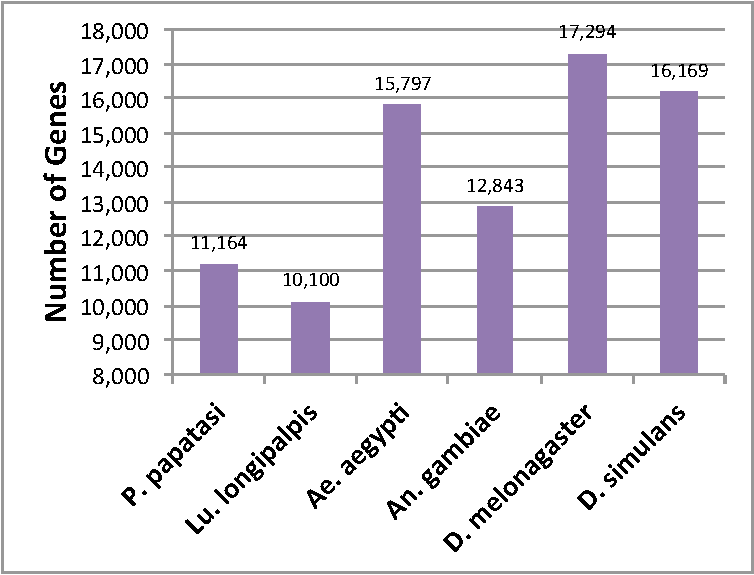
\includegraphics[width=\textwidth]{figures/synteny/genome_size_genes.pdf}
    \caption{Genome Sizes (Genes)}
    \label{fig:number-genes}
  \end{subfigure}
  ~
  \begin{subfigure}[b]{0.45\textwidth}
    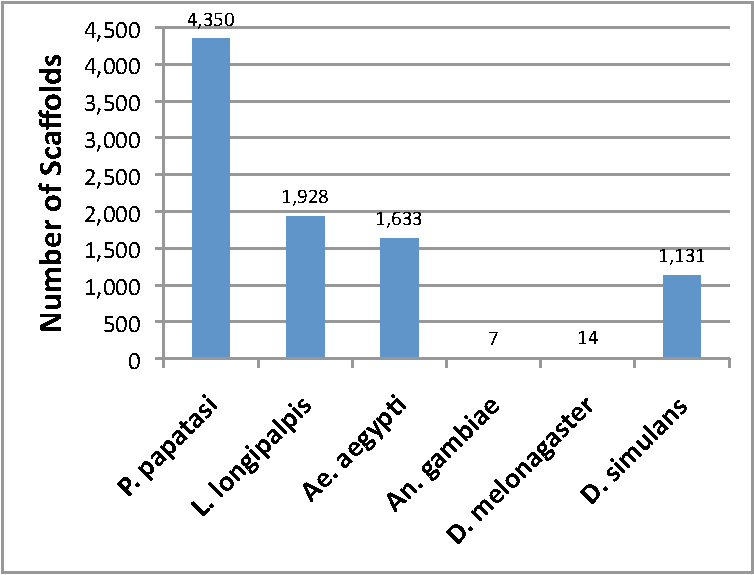
\includegraphics[width=\textwidth]{figures/synteny/scaffold_counts.pdf}
    \caption{Number of Scaffolds}
    \label{fig:number-scaffolds}
  \end{subfigure}
  ~
  \begin{subfigure}[b]{0.45\textwidth}
    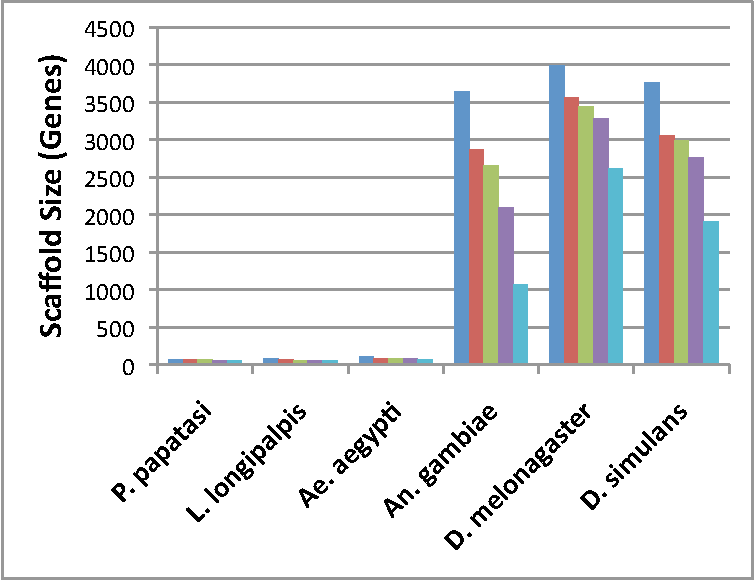
\includegraphics[width=\textwidth]{figures/synteny/top5_scaffold_sizes.pdf}
    \caption{Top 5 Scaffold Sizes (Genes)}
    \label{fig:largest-scaffolds}
  \end{subfigure}
  ~
  \begin{subfigure}[b]{0.45\textwidth}
    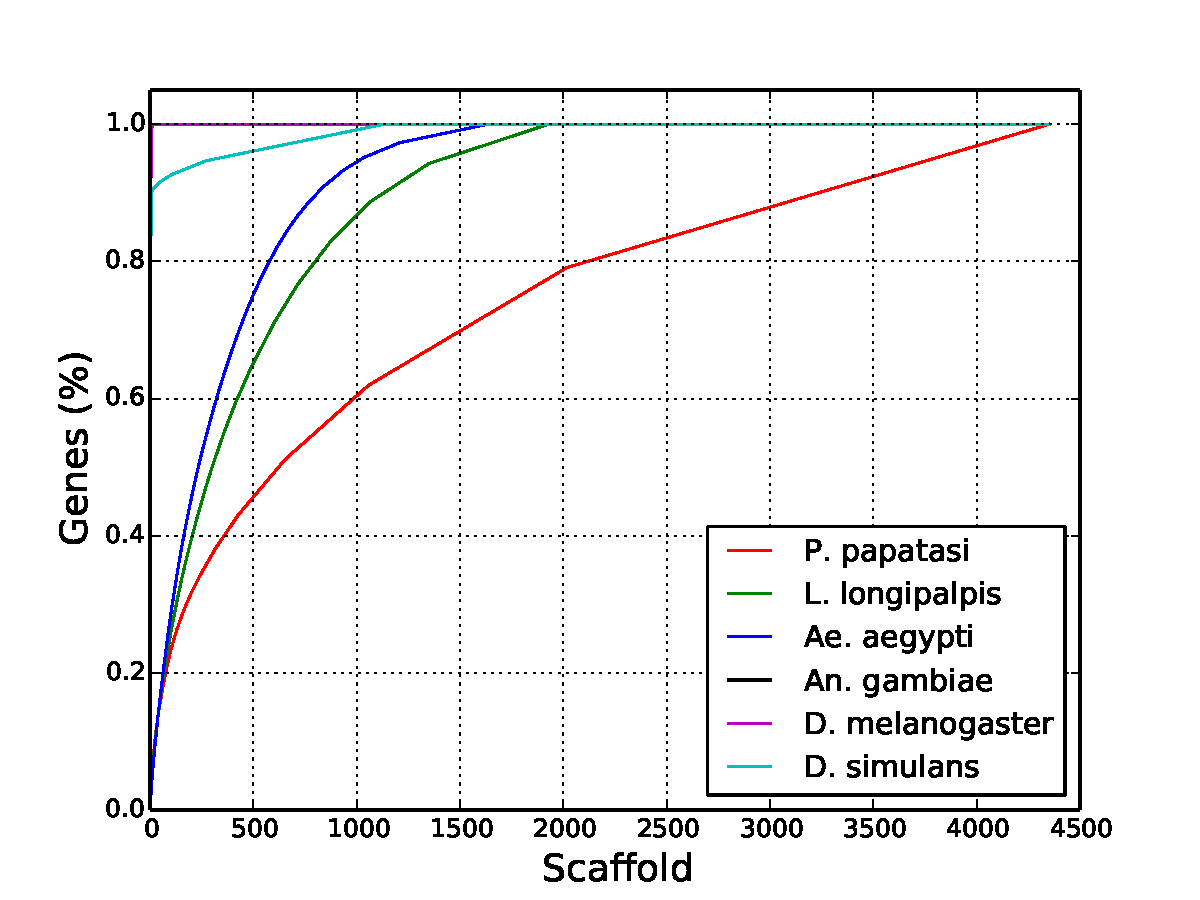
\includegraphics[width=\textwidth]{figures/synteny/gene_scaffold_cdf.pdf}
    \caption{Cumulative Distribution of Genes over Scaffolds}
    \label{fig:gene-scaffold-cdf}
  \end{subfigure}
  \label{fig:scaffolds}
\end{figure}


\begin{table}[H]
  \begin{center}
  \small
  \caption{\label{tab:scaffold-sizes} SCAFFOLD SIZE STATISTICS}
  \begin{tabular}{c p{1.25cm} p{1.25cm} c p{1.25cm} p{1.25cm} p{1.25cm} p{1.25cm}} \hline
    \emph{Species} & \emph{Genome Size (Mbp)} & \emph{Scaffold N50 (Mbp)} & \emph{Scaffolds} & \emph{Scaffold Size (Genes)} & \emph{Average} & \emph{Median} & \emph{Max.} \\ \hline
    \emph{Ae. aegypti} & 1,310.0 & 1.6 & 1,633 & 15,797 & 9.7 & 5 & 104 \\
    \emph{An. gambiae} & 278.3 & 49.4 & 7 & 12,843 & 1,834.7 & 2,093 & 3,684 \\
    \emph{D. melonagaster} & 143.7 & & 14 & 17,294 & 1,235.3 & 74 & 3,991 \\ 
    \emph{D. simulans} & 153.1 & & 1,131 & 16,196 & 14.3 & 1 & 3,767 \\ 
    \emph{Lu. longipalpis} & 154.2 & 13.9 & 1,928 & 10,100 & 5.2 & 1 & 73\\
    \emph{P. papatasi} & 347.8 & 17.6 & 4,350 & 11,164 & 2.6 & 1 & 84
  \end{tabular}
  \end{center}
  \tablenote{Genome sizes for \emph{D. melonagaster} and \emph{D. simulans} are from Ensembl \cite{Hubbard2002} and from Vectorbase \cite{Lawson2009,Lawson2007} for other species. Size statistics for the scaffolds are given in numbers of genes.}
\end{table}

\subsection{Conservation of Gene Order (Synteny)}
Rearrangements of chromosomes are rare events and tend to happen in a block-wise fashion that mainly preserves the local order of genes on the chromosome. Thus, even after long periods of divergence between species, synteny blocks, defined as conserved runs of consecutive orthologous genes, remain discernible \cite{Heger2007}.  The presence of synteny can be used to infer evolutionary relationships between organisms' genomes at a macroscopic level, complementing analyses such as gene family expansions and reductions and changes within pairs of orthologous genes \cite{Zdobnov2002,Zdobnov2007}.

We did not observe the presence of macrosynteny between the \emph{Lu. longipalpis} and \emph{P. papatasi} genomes (Figure~\ref{fig:synteny-dotplots-sandflies}).  Synteny analysis is dependent on the completeness of genome assemblies \cite{Heger2007}; the sizes of synteny blocks are naturally bounded by the size of the largest scaffolds (73 genes for \emph{Lu. longipalpis} and 84 genes for \emph{P. papatasi}). Macrosynteny was also absent in the comparison of \emph{An. gambiae} and \emph{D. melanogaster}, whose genome assemblies are complete to the level of chromosomes but present between the \emph{D. melanogaster} and \emph{D. simulans} (Figure~\ref{fig:synteny-dotplots-drosophila}), which are more closely-related than any other pair of species we have analyzed. There simply may not be macrosynteny given the high rate of genome shuffling observed in insect genomes and the evolutionary distances of the species under comparison. Comparative studies of synteny and gene order between insect genomes (e.g., \emph{Drosophila}) have indicated significant levels of genome shuffling, more so than observed in fish and humans \cite{Ranz2001,Zdobnov2002,Zdobnov2007}.

\begin{figure}[H]
  \centering
  \caption{Qualitative Analysis of Macrosynteny}
  \begin{subfigure}[b]{0.4\textwidth}
    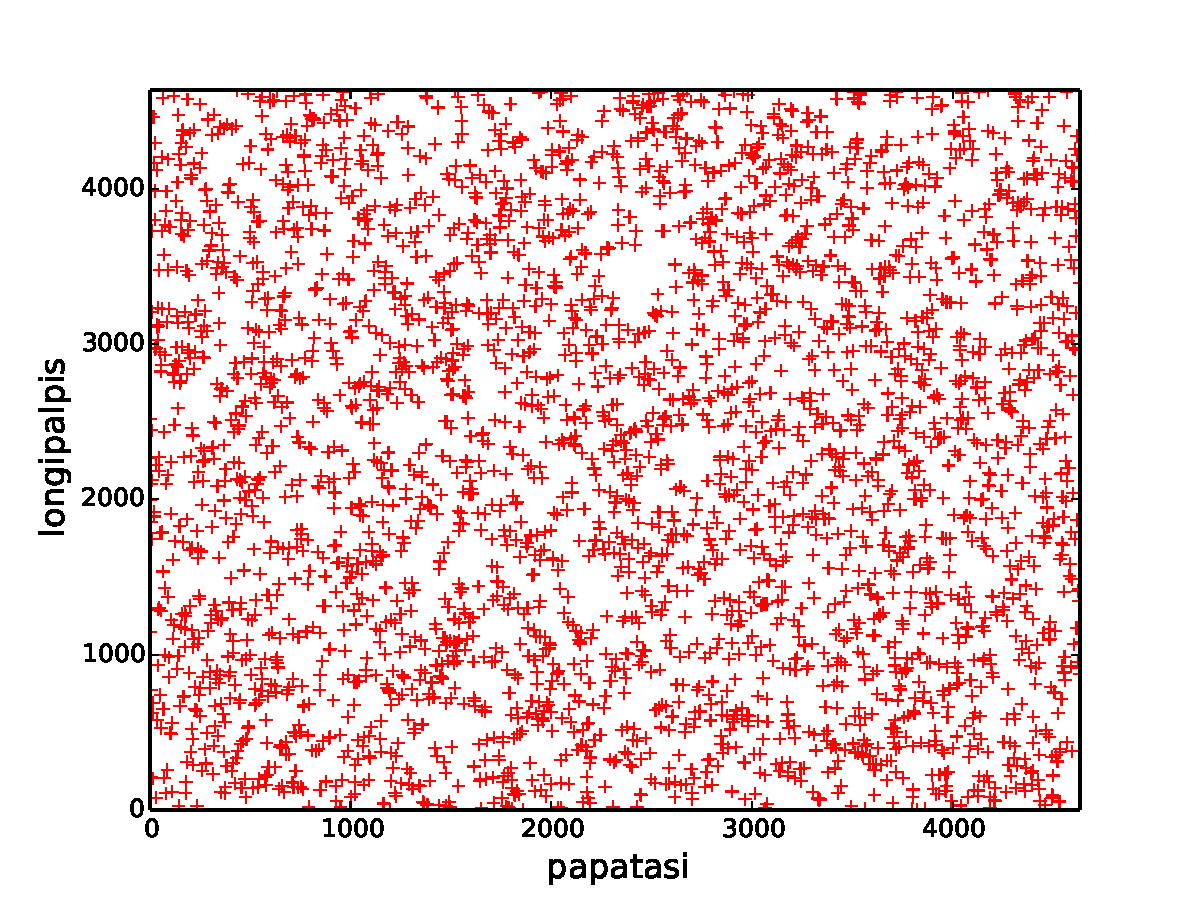
\includegraphics[width=\textwidth]{figures/synteny/papatasi_longipalpis_plot}
    \caption{\label{fig:synteny-dotplots-sandflies}}
  \end{subfigure}
  \\
  \begin{subfigure}[b]{0.4\textwidth}
    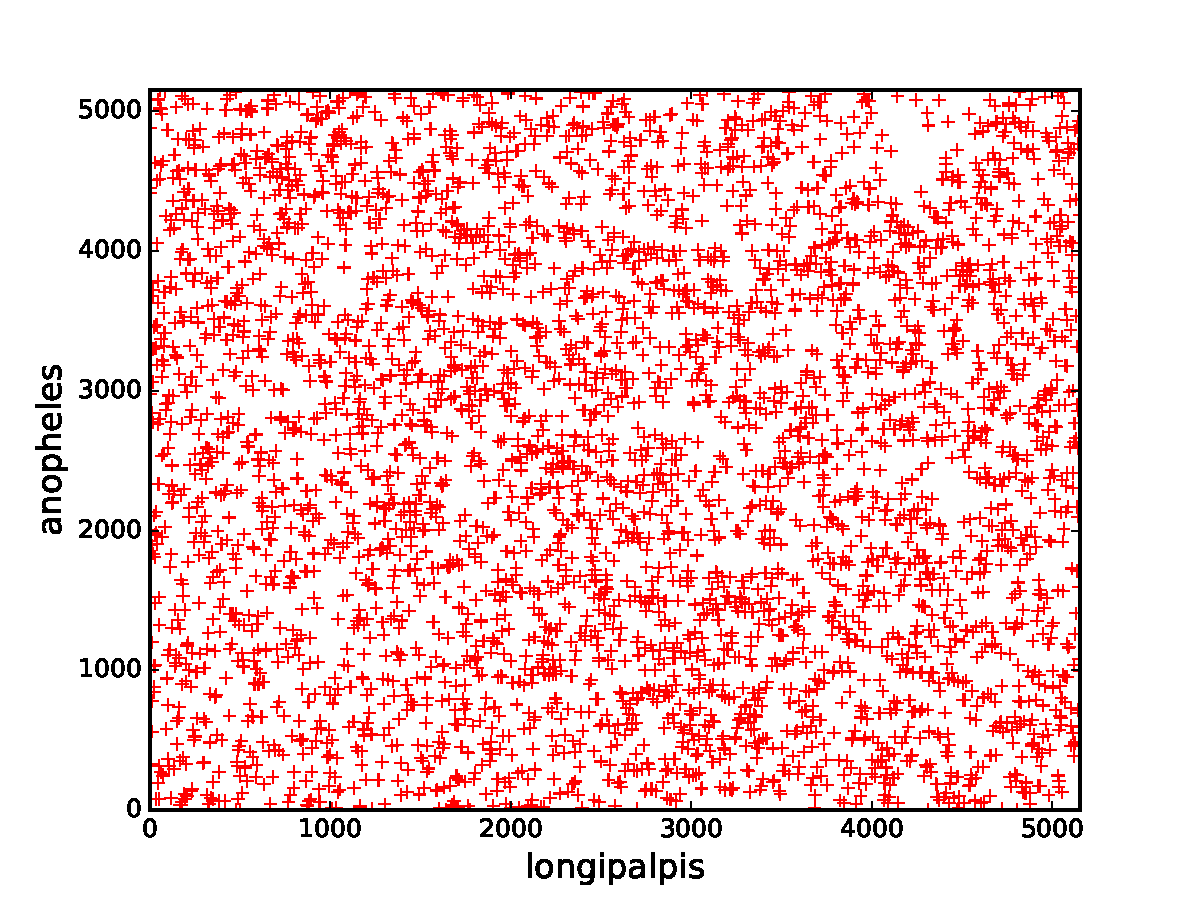
\includegraphics[width=\textwidth]{figures/synteny/longipalpis_anopheles_plot}
    \caption{\label{fig:synteny-dotplots-longipalpis-anopheles}}
  \end{subfigure}
  ~
  \begin{subfigure}[b]{0.4\textwidth}
    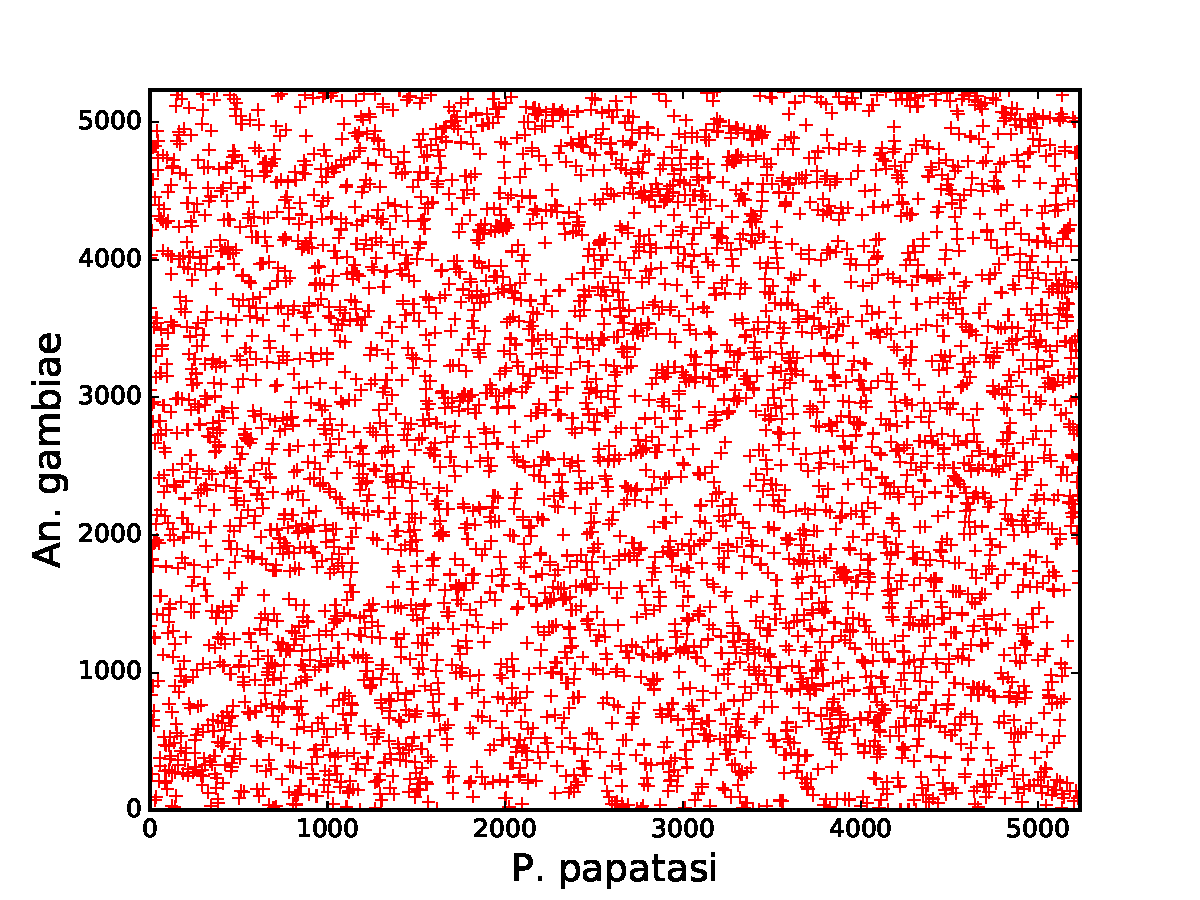
\includegraphics[width=\textwidth]{figures/synteny/papatasi_anopheles_plot}
    \caption{\label{fig:synteny-dotplots-papatasi-anopheles}}
  \end{subfigure}
  ~
  \begin{subfigure}[b]{0.4\textwidth}
    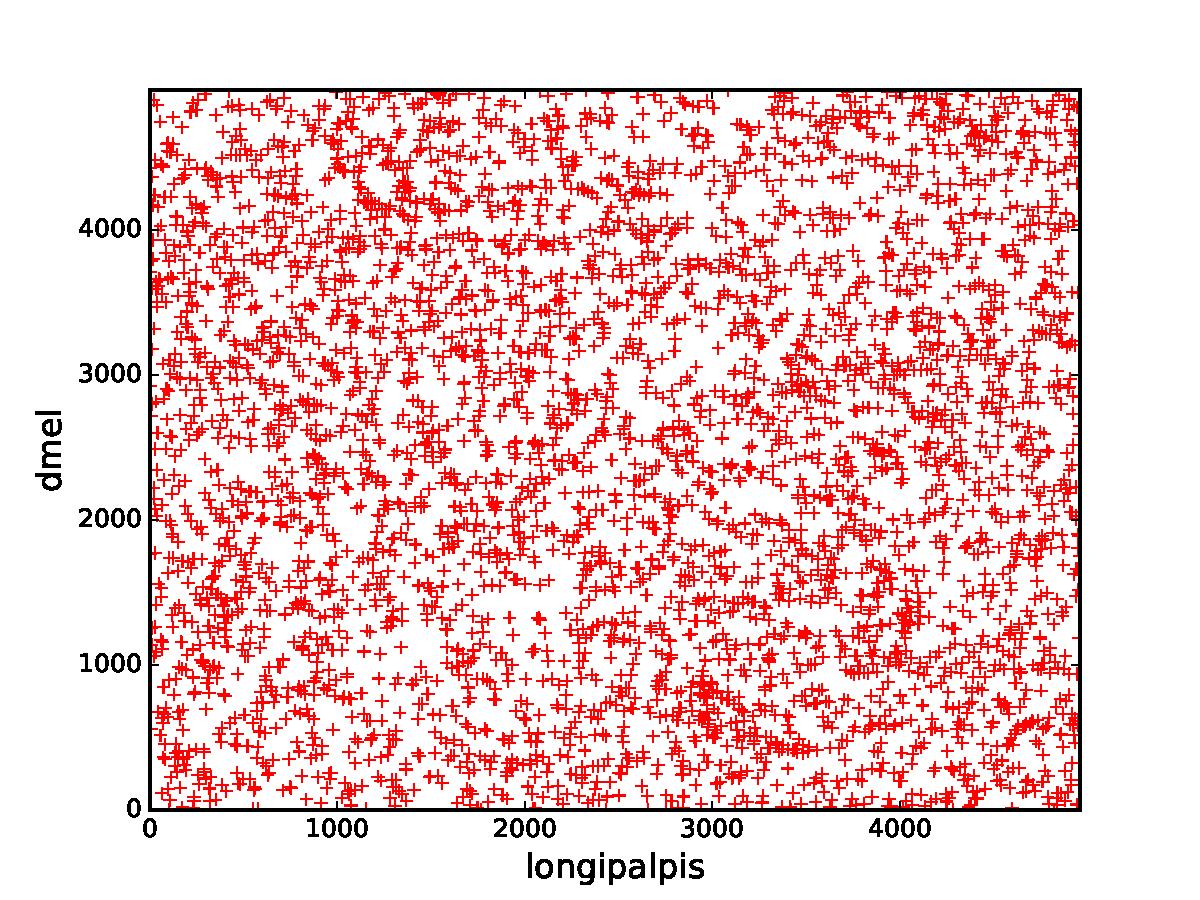
\includegraphics[width=\textwidth]{figures/synteny/longipalpis_dmel_plot}
    \caption{\label{fig:synteny-dotplots-longipalpis-dmel}}
  \end{subfigure}
  ~
  \begin{subfigure}[b]{0.4\textwidth}
    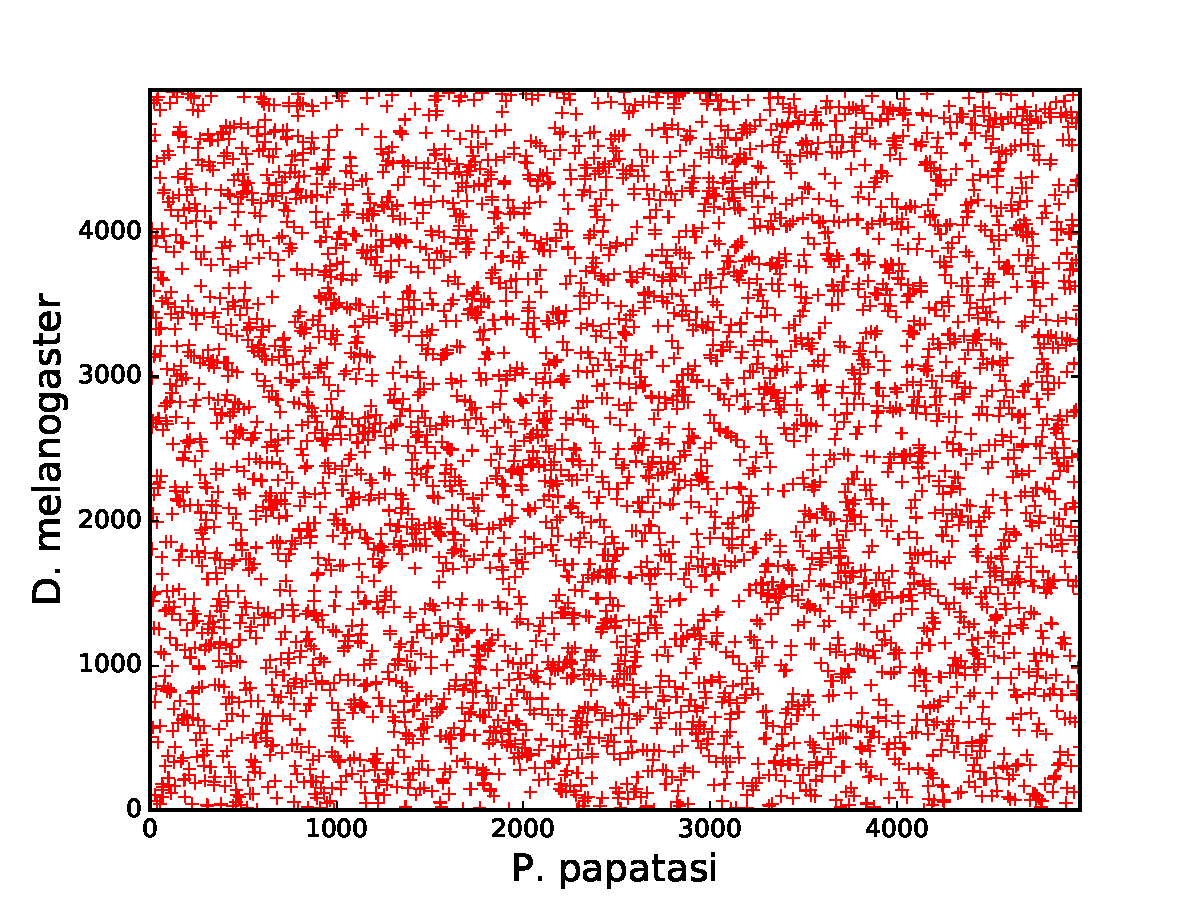
\includegraphics[width=\textwidth]{figures/synteny/papatasi_dmel_plot}
    \caption{\label{fig:synteny-dotplots-papatasi-dmel}}
  \end{subfigure}
\end{figure}

\begin{figure}[H]
  \ContinuedFloat
  \centering
  \caption{Qualitative Analysis of Macrosynteny (cont).}
  \begin{subfigure}[b]{0.4\textwidth}
    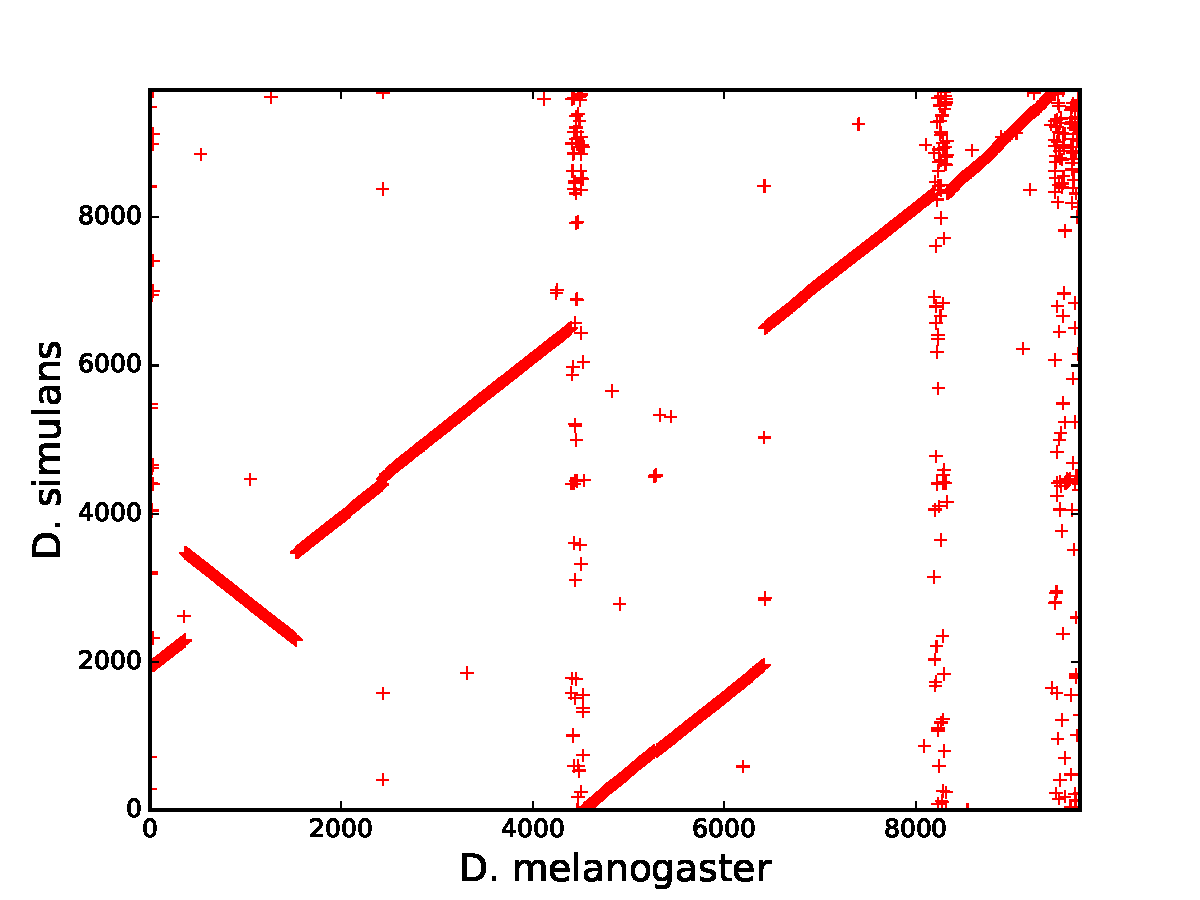
\includegraphics[width=\textwidth]{figures/synteny/dmel_dsim_plot}
    \caption{\label{fig:synteny-dotplots-drosophila}}
  \end{subfigure}
  ~
  \begin{subfigure}[b]{0.4\textwidth}
    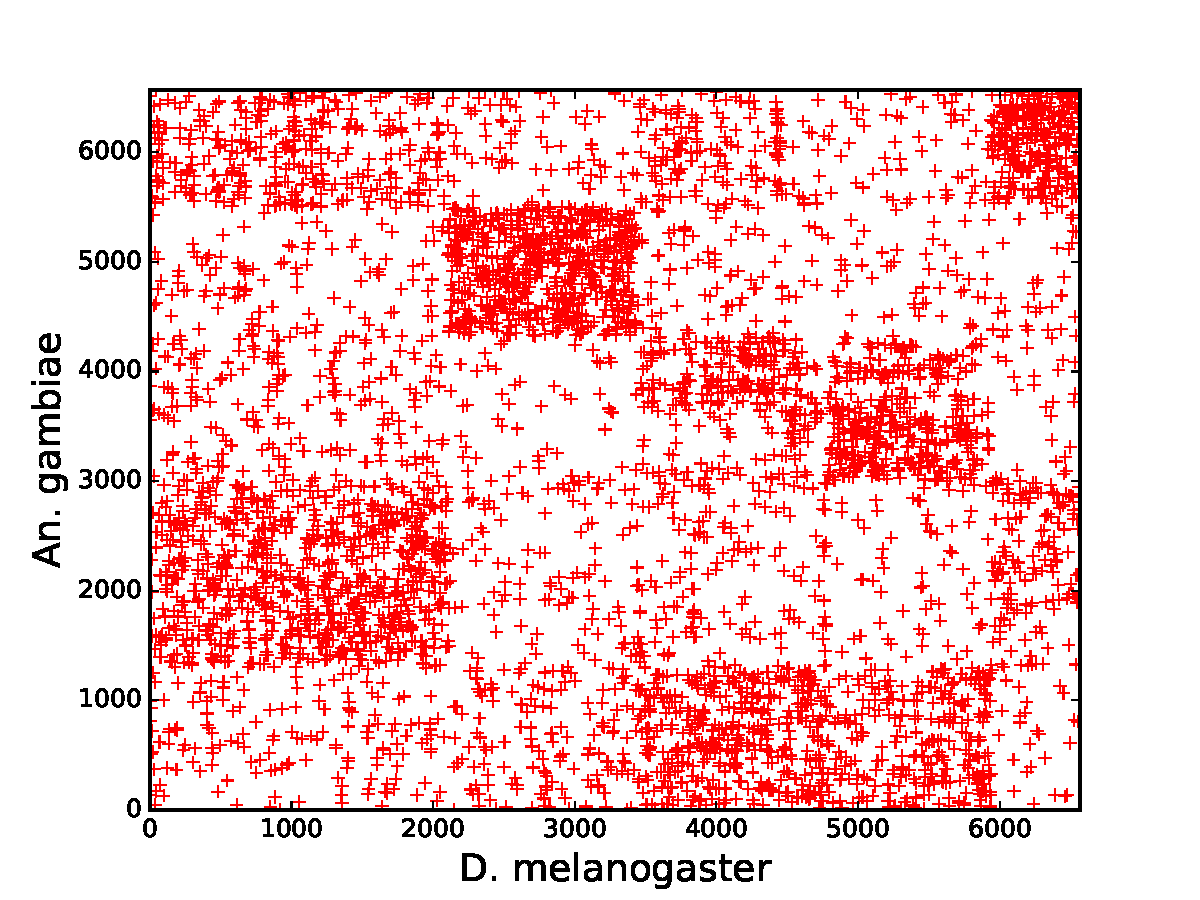
\includegraphics[width=\textwidth]{figures/synteny/dmel_anopheles_plot}
    \caption{\label{fig:synteny-dotplots-anopheles-drosophila}}
  \end{subfigure}
  \label{fig:dot-plots}

  Scatter plots of ortholog locations in each pair of genomes. The lines in (f), but absent from the other comparisons, are evidence for macrosynteny.
\end{figure}

Microsynteny was, however, observed between the sand flies species and each species with \emph{An. gambiae} (Table~\ref{tab:synteny-block-stats}). Microsynteny between \emph{Lu. longipalpis} and \emph{P. papatasi} is on-par with the microsynteny we observed and previously reported by others for \emph{An. gambiae} and \emph{D. melonagaster}.  Between the \emph{Lu. longipalpis} and \emph{P. papatasi} genomes, we identified a total of 499 synteny blocks with a maximum of 24 genes, average of 4.2 genes, and a median of 3 genes. By comparison, between the genomes of \emph{An. gambiae} and \emph{D. melonagaster}, we found 1,037 synteny blocks with a maximum of 10 genes, an average of 2.5 genes, and a median of 2 genes. Previous studies of \emph{An. gambiae} and \emph{D. melonagaster} reported a similar number of synteny blocks (948) with up to 39 genes \cite{Zdobnov2002}.

\begin{table}[H]
  \begin{center}
    \small
  \caption{\label{tab:synteny-block-stats} MICROSYNTENY BLOCK STATISTICS}
  \begin{tabular}{c c p{1cm} c c} \hline
    \emph{Species} & \emph{Count} & \emph{Average Size} & \emph{Median Size} & \emph{Max. Size} \\ \hline
    \emph{Lu. longipalpis} vs. \emph{An. gambiae} & 504 & 4.3 & 3 & 39 \\
    \emph{Lu. longipalpis} vs. \emph{P. papatasi} & 499 & 4.2 & 3 & 24 \\
    \emph{P. papatasi} vs. \emph{An. gambiae} & 307 & 4.3 & 3 & 21 \\
    \emph{D. melanogaster} vs. \emph{D. simulans} & 243 & 41.6 & 5 & 700 \\
    \emph{D. melanogaster} vs. \emph{An. gambiae} & 1037 & 2.5 & 2 & 10
  \end{tabular}
  \end{center}
  \tablenote{Sizes are given in number of genes.}
\end{table}

Microsynteny is more robust to genome assembly fragmentation and expected in organisms with the evolutionary distances of the sand flies and \emph{An. gambiae} \cite{Zdobnov2002}. Noncoding elements, particularly associated with gene regulation, have been found to be highly-conserved in insect microsynteny blocks, suggesting a cause for the preservation of small-scale gene order \cite{Engstrom2007}.

We annotated and analyzed the largest synteny blocks from \emph{Lu. longipalpis} and \emph{P. papatasi} and a three-way comparison of \emph{An. gambiae}, \emph{Lu. longipalpis}, and \emph{P. papatasi}.  Four of the largest synteny blocks from \emph{Lu. longipalpis} and \emph{P. papatasi} contained peritrophin-like, membrane-bound or -associated, RNA regulation and synthesis, and intracellular processes genes. The largest synteny blocks between \emph{An. gambiae}, \emph{Lu. longipalpis}, and \emph{P. papatasi} contained genes associated with the dopamine signaling pathway and enzyme regulation, sterol homeostatis and steroid biosynthesis (Niemann-Pick type C-2), transcription regulation and protein modification, and amino acid transport and protein modification.

\subsection{Comparison of Protein Sequence Identity with $d_N$/$d_S$}
Evolutionary changes at the level of individual genes were analyzed through comparing distributions of $d_N$/$d_S$ ratios of single-copy orthologs. DNA base pairs are subject to random substitutions as organisms reproduce.  Substitutions in protein-coding open-reading frames can be divided into two types: synonymous (silent) mutations which do not affect the resulting amino acid sequences and non-synonymous (non-silent) mutations which do affect the resulting amino acid sequences and can affect gene function.  Silent mutations are assumed not to be under any sort of selection process, correlating with an organism's rate of evolutionary change.  Non-silent mutations are less likely to be passed on since they may impair the function of important genes; those that are inherited either do not impact gene function or are under selection pressure as an organism adapts.

The $d_N$/$d_S$ ratio measures the rate of synonymous substitutions ($d_S$), which are presumed neutral, to the rate of non-synonymous substitutions ($d_N$) \cite{Kryazhimskiy2008}. Genes with $d_N$/$d_S$ $>$ 1 have non-silent substitutions at a higher rate than the background rate of the organism's evolutionary change would suggest.  As such, these genes are assumed to be under positive selection pressure.  Genes with $d_N$/$d_S$ $<1$ have fewer non-silent substitutions, suggesting purifying selection pressure and greater conservation in their sequences.

We analyzed $d_N$/$d_S$ ratios between single-copy orthologs in pairwise comparisons of the sand flies \emph{Lu. longipalpis} and \emph{P. papatasi}, mosquito \emph{An. gambiae}, and fruit fly \emph{D. melanogaster}.  The distributions of $d_N$/$d_S$ ratios are given in Figure~\ref{fig:dnds-distr}.  Except for the comparison between \emph{Lu. longipalpis} and \emph{P. papatasi}, the distributions are remarkedly similar.

\begin{figure}[H]
  \centering
  \caption{Distribution of $d_N$/$d_S$ Ratios}
  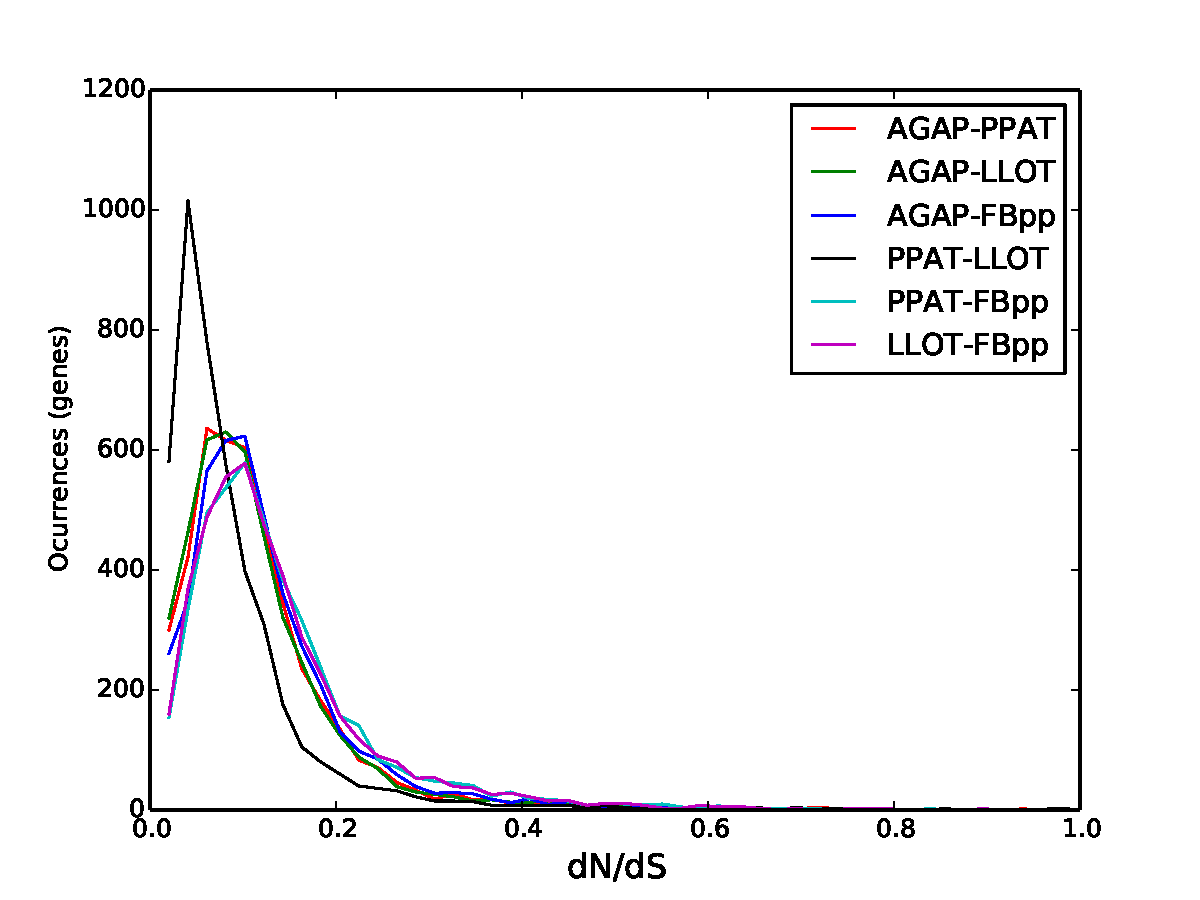
\includegraphics[width=0.75\textwidth]{figures/ka_ks/dN_dS}
  \label{fig:dnds-distr}

  Distributions of $d_N$/$d_S$ ratios were computed pairwise for \emph{An. gambiae} (AGAP), \emph{D. melanogaster} (FBpp), \emph{Lu. longipalpis} (LLOT), and \emph{P. papatasi} (PPAT). A small number of orthologs had $d_N$/$d_S$ ratios $>1$ and are not shown in the plot.
\end{figure}


The $d_N$/$d_S$ distribution for single-copy orthologs from \emph{Lu. longipalpis} and \emph{P. papatasi} is skewed towards zero when compared with distributions with and between \emph{An. gambiae} and \emph{D. melanogaster}.  The smaller $d_N$/$d_S$ values indicate fewer non-silent substitutions relative to the number of silent substitutions.  The smaller values could be a result of the shorter evolutionary distance between \emph{Lu. longipalpis} and \emph{P. papatasi} versus any other pair of species we compared.  However, we also found, in line with the fragmentation of the genome assemblies, that many gene models are shorter than their orthologs in other species, indicating that the gene models may not be complete (results not shown).  Thus, the lower $d_N$/$d_S$ values could also caused by truncated gene models that contain only the most conserved segments of genes.

\subsection{Differential Gene Expression in Sugar-Fed, Blood-Fed, and Infected Blood-Fed \emph{Lu. longipalpis} Females}
RNASeq differental gene expression data was collected from \emph{Lu. longipalpis} females 6, 24, and 144 hours after being fed sugar, bloodmeals, and bloodmeals infected with the leishmaniasis parasite, \emph{Leishmania infantum}.  We identified a total of 6,979 genes with statistically-significant differences in expression between blood-fed and sugar-fed females over the three time points (see Table~\ref{tab:stat-sig-genes}).  Fewer genes (3,822) had statistically-significantly differences in expression when compared between blood-fed and infected blood-fed females.

\begin{table}[H]
  \begin{center}
    \small
  \caption{\label{tab:stat-sig-genes} \uppercase{Number of Genes with Statistically-Significant Differential Expression}}
  \begin{tabular}{c c c} \hline
  \emph{Time Point} & \emph{Blood Fed vs Sugar Fed} & \emph{Infected Blood Fed vs Blood Fed} \\ \hline
  6H & 4,062 & 1,332 \\
  24H & 4,486 & 2,483 \\
  144H & 5,209 & 1,410 \\
  \end{tabular}
  \end{center}
\end{table}

Comparison of GO-slim term distributions yielded little insight into differences in expression between the conditions due to the overwhelming number of genes with statistically-significant differences in expression.  As such, we focused on comparing expression of genes from families and pathways associated with immunity between blood fed and infected blood fed conditions.

\subsection{Peritrophins}
Host-parasite interactions are of particular interest.  Within a few hours, a peritrophic matrix forms around the blood bolus.  The peritrophic matrix thickens and matures around 12 to 24 hours, depending on the sand fly species.  After 48 to 72 hours, the peritrophix matric structure starts to break down.  The peritrophic matrix seems to play a dual role with respect to \emph{Leishmania} development: the peritrophic matrix protects the parasite against attack by proteolytic proteins at the beginning of digestion yet becomes a barrier to parasite escape when mature \cite{Pimenta1997,Dostalova2012}.

We analyzed differences in expression of peritrophins between sugar-fed and blood-fed conditions and blood-fed and infected blood-fed conditions.  Due to data quality issues, CuffDiff only performed statistical tests on 8 of the 28 identified of the peritrophins (see Tables~\ref{tab:sandflies:stat-sig-peritrophins-sb}~and~\ref{tab:sandflies:stat-sig-peritrophins-bi}).  LuloPer4 (LLOTMP003410), LuloPer10 (LLOTMP007615), and LuloPer11 (LLOTMP002676) had no statistically-significant differences at two or more time points.

\begin{table}[H]
  \begin{center}
    \small
  \caption{\label{tab:sandflies:stat-sig-peritrophins-sb} PERITROPHIN EXPRESSION (BLOOD-FED VS. SUGAR-FED)}
  \begin{tabular}{ c c c c c } \hline
    \emph{Gene} & \emph{Identifier} & \emph{6 hours} & \emph{24 hours} & \emph{144 hours} \\ \hline
    LuloPer1 & LLOTMP006497 & Yes (3.96028) & Yes (10.5884) & No \\
    LuloPer2 & LLOTMP003676 & Yes (0.41318) & Yes (1.61758) & Yes (-0.608263) \\
    LuloPer3b & LLOTMP004906 & Yes (1.32142) & Yes (0.940809) & Yes (0.603129) \\
    LuloPer32 & LLOTMP004516 & Yes (-0.985627) & Yes (2.27779) & Yes (-2.2308)
  \end{tabular}
  \end{center}
  \tablenote{Peritrophins with statistically-significant differences in expression between sugar fed and blood fed conditions. Log-fold change is given in parentheses. Positive and negative values indicate up- and down-regulation in blood fed, respectively.}
\end{table}

\begin{table}[H]
  \begin{center}
    \small
  \caption{\label{tab:sandflies:stat-sig-peritrophins-bi} PERITROPHIN EXPRESSION (INFECTED BLOOD-FED VS. BLOOD-FED)}
  \begin{tabular}{ c c c c c } \hline
    \emph{Gene} & \emph{Identifier} & \emph{6 hours} & \emph{24 hours} & \emph{144 hours} \\ \hline
    LuloPer1 & LLOTMP006497 & Yes (1.2595) & Yes (0.384657) & No \\
    LuloPer2 & LLOTMP003676 & No & Yes (0.183758) & Yes (-0.684151) \\
    LuloPer3a & LLOTMP002647 & Yes (0.283665) & Yes (0.152629) & Yes (0.358638) \\
    LuloPer3b & LLOTMP004906 & Yes (-0.137809) & Yes (1.20303) & No \\
    LuloPer32 & LLOTMP004516 & Yes (1.14581) & Yes (0.612843) & No
  \end{tabular}
  \end{center}
  \tablenote{Peritrophins with statistically-significant differences in expression between blood fed and infected blood fed conditions. Log-fold change is given in parentheses. Positive and negative values indicate up- and down-regulation in infected blood fed, respectively.}
\end{table}

A previous EST (expression tag sequence) study reported increased expression of LuloPer1 (LLOTMP006497), LuloPer2 (LLOTMP003676), and LuloPer32 (LLOTMP004516) after blood feeding \cite{Jochim2008}. Similarly, we observed up-regulation of LuloPer1, LuloPer2, and LuloPer32 at 24 hours after blood-feeding, after the peritrophic matrix thickens and matures.  We also observed increased expression of LuloPer1 and LuloPer2 but decreased expression of LuloPer32 at 6 hours, prior to the maturation of the peritrophic matrix. At 144 hours, after the peritrophic matrix starts to degrade, we observed down-regulation of LuloPer2 and LuloPer32 but no change in expression of LuloPer1.

Differential expression of LuloPer1 was observed to be increased with infected blood feeding at 6 and 24 hours, in agreement with the EST data \cite{Jochim2008,Dostalova2012}.  However, while the EST data showed no significant difference in expression under infection, we observed an increase in the expression of LuloPer32 at 6 and 24 hours and LuloPer2 at 6 hours followed by a decrease in expression at 24 hours \cite{Jochim2008}.  At 144 hours, LuloPer2 was down-regulated but LuloPer1 and LuloPer32 had no change in expression.

Differential expression levels of LuloPer3a (LLOTMP002647) and LuloPer3b (LLOTMP004906) were observed in the RNASeq analysis but were not found in the EST expression analysis \cite{Jochim2008}. LuloPer3b was up-regulated in blood fed (vs sugar fed) across all three time points and down-regulated at 6 hours and up-regulated at 24 hours in infected blood fed (vs sugar fed) conditions.  Expression of LuloPer3a had no statistically-significantly difference between blood fed and sugar fed conditions but was up-regulated across all three time points under infected bood fed (vs blood fed) conditions.

The RNASeq differential expression analysis confirmed the previous EST expression analysis of LuloPer1, LuloPer2, and LuloPer32 under blood fed (vs sugar fed) conditions and LuloPer1 under infected blood fed (vs blood fed) conditions.  We found differences in the expression of LuloPer2 and LuloPer32 under infected blood fed (vs blood fed) conditions, which had not been observed previously \cite{Jochim2008,Dostalova2012}.  We also observed previously-unreported statistically-significant differences in expression of LuloPer3b under blood-fed (vs sugar-fed) conditions and LuloPer2 and LuloPer3b under infected blood-fed (vs blood-fed) conditions. Further analysis is needed to determine the exact functions of the peritrophins and the importance of the observed expression profiles.

LuloPer1 and four peritropins without RNASeq results are located in a microsynteny block from \emph{Lu. longipalpis} and \emph{P. papatasi} (see Table~\ref{tab:synteny-llot-ppat-peritrophic}). As previously noted, highly-conserved noncoding elements, particularly associated with gene regulation, have been found previously in insect microsynteny blocks \cite{Engstrom2007}.  Further study of peritrophins could potentially lead to  better understanding the relationship between regulation mechanisms and microsynteny in general and the molecular mechanisms of the peritrophin's regulation specifically.

\begin{table}[H]
  \begin{center}
  \small
  \caption{\label{tab:synteny-llot-ppat-peritrophic} PERITROPHIN MICROSYNTENY BLOCK}
  \begin{tabular}{c c l} \hline
    \emph{Lu. longipalpis} & \emph{P. papatasi} & \emph{Description} \\ \hline
    LLOTMP006493 & PPATMP009348 & SCP-related protein \\
    LLOTMP006494 & PPATMP009349 & ribosomal protein S23 \\
    LLOTMP006495 & PPATMP009350 & LuloPer22 \\
    LLOTMP006496 & PPATMP009351 & LuloPer14 \\
    LLOTMP006497 & PPATMP009352 & LuloPer1 \\
    LLOTMP006498 & PPATMP009353 &  \\
    LLOTMP006499 & PPATMP009355 & LuloPer18 \\
    LLOTMP006500 & PPATMP009356 & LuloPer17
  \end{tabular}
  \end{center}
  \tablenote{Synteny block of peritrophins from \emph{Lu. longipalpis} vs. \emph{P. papatasi}.}
\end{table}


\subsection{Chitinases}
The breakdown of the peritrophic matrix has been attributed to chitinases \cite{Dostalova2012}. Eleven chitinase genes have been identified in the \emph{Lu. longipalpis} genome. Due to data quality issues, CuffDiff could not perform statistical tests on two of the genes, cht12 like protein (LLOTMP003713) and Llcht5 (LLOTMP008303). Llcht7 (LLOTMP009389) and Llcht8 (LLOTMP003119) did not have statistically-significant differences in expression for more than one time point in comparisons of blood-fed vs sugar-fed or blood-fed vs blood-fed infected conditions.

In a comparison of blood fed to sugar fed conditions, only two of the chitinases were up-regulated (see Table~\ref{tab:sandflies:stat-sig-chitinases-sb}): Llcht1/midgut cht (LLOTMP000006) and Llcht8 (LLOTMP003119) were up-regulated at 6 and 24 hours, with Llcht1/midgut cht up-regulated and Llcht8 down-regulated at 144 hours.  Llcht1 was previously found to be up-regulated under blood fed vs sugar fed conditions, peaking at 72 hours \cite{Ramalho-Ortigao2003}. Neither Llcht1 nor Llcht8 had statistically-significant differences in expression levels between blood-fed and blood-fed infected conditions at any time points. RNA interference knock-down of PpChit1 (an ortholog of of Llcht1) in \emph{P. papatasi} fed \emph{Le. major}-infected bloodmeals has been observed to be associated with a significantly reduction in the number of parasites present in the midgut 120 hours after the bloodmeal \cite{Coutinho-abreu2010}, suggesting that the degradation of the PM by PpChit1 enables the escape of the parasites.  Further analysis is needed to confirm a similar role for Llcht1 in \emph{Lu. longipalpis}. 

Five chitinases were down-regulated under blood fed vs sugar fed conditions at all time points for which differences were statistically significant: LlIDGF4 (LLOTMP008789), LlIDGF4 (LLOTMP004095), chitinase like protein (LLOTMP006041), Llcht10 (LLOTMP006362), and Llcht2 (LLOTMP008646).  In the comparisons of blood-fed vs blood-fed infected conditions, no statistically-significant differences in expression were observed for LlIDGF4 (LLOTMP008789) and Llcht2 and CuffDiff was not able to perform statistical tests on Llcht10 for two of the time points and no statistically-significant difference was found at the third time point. LlIDGF4 (LLOTMP004095) and chitinase like protein (LLOTMP006041) were the only chitinases with statistically-significant differences in expression in blood-fed vs infected blood-fed conditions (see Table~\ref{tab:sandflies:stat-sig-chitinases-bi}); both were up-regulated at 6 and 24 hours, while at 144 hours, chitinase like protein (LLOTMP006041) was still up-regulated but LlIDGF4 (LLOTMP004095) had no statistically-significant difference. Further work is needed to understand the the role and cause of up-regulation of LlIDGF4 (LLOTMP004095) and chitinase like protein (LLOTMP006041) in the presence of \emph{Leishmania}.

\begin{table}[H]
  \begin{center}
  \caption{\label{tab:sandflies:stat-sig-chitinases-sb} CHITINASE EXPRESSION (BLOOD-FED VS. SUGAR-FED)}
  \begin{tabular}{ c c c c c } \hline
    \emph{Gene} & \emph{Identifier} & \emph{6 hours} & \emph{24 hours} & \emph{144 hours} \\ \hline
    LlIDGF4 & LLOTMP008789 & Yes (-0.391866) & Yes (-0.286923) & Yes (-0.547106) \\
    LlIDGF4 & LLOTMP004095 & Yes (-1.53121) & Yes (-1.70157) & Yes (-1.18189) \\
    Llcht1/midgut cht & LLOTMP000006 & Yes (0.423869) & Yes (0.704253) & Yes (-0.896378) \\
    chitinase like protein & LLOTMP009205 & Yes (0.642386) & Yes (0.495779) & Yes (0.687019) \\
    chitinase like protein & LLOTMP006041 & Yes (-1.02214) & No & Yes (-1.31797) \\
    Llcht10 & LLOTMP006362 & Yes (-0.475676) & No & Yes (-1.04283) \\
    Llcht2 & LLOTMP008646 & Yes (-0.778297) & Yes (-1.14975) & Yes (-1.93176)
  \end{tabular}
  \end{center}
  \tablenote{Chitinases with statistically-significant differences in expression between sugar fed and blood fed conditions. Log-fold change is given in parentheses. Positive and negative values indicate up- and down-regulation in blood fed, respectively.}
\end{table}

\begin{table}[H]
  \begin{center}
  \caption{\label{tab:sandflies:stat-sig-chitinases-bi} CHITINASE EXPRESSION (INFECTED BLOOD-FED VS. BLOOD-FED)}
  \begin{tabular}{ c c c c c } \hline
    \emph{Gene} & \emph{Identifier} & \emph{6 hours} & \emph{24 hours} & \emph{144 hours} \\ \hline
    LlIDGF4 & LLOTMP004095 & Yes (0.654322) & Yes (0.56086) & No \\
    chitinase like protein & LLOTMP006041 & Yes (0.532128) & Yes (0.559772) & Yes (0.4717)
  \end{tabular}
  \end{center}
  \tablenote{Chitinases with statistically-significant differences in expression between blood fed and infected blood fed conditions. Log-fold change is given in parentheses. Positive and negative values indicate up- and down-regulation in infected blood fed, respectively.}
\end{table}


\subsection{Niemann Pick Type C-2 (NPC2) Genes}
A three-way comparison of synteny between \emph{An. gambiae}, \emph{Lu. longipalpis}, and \emph{P. papatasi} revealed a block of Niemann Pick type C2 (NPC2) genes (Table~\ref{tab:synteny-three-way-npc2}). In insects, NPC genes are involved with sterol (e.g., cholesterol) homeostasis and biosynthesis of ecdysteroids, insect sex and moulting hormones. In humans, mutations in either of two Niemann Pick type C (NPC) genes, \emph{NPC1} and \emph{NPC2}, cause a fatal neurogenerative disorder associated with abnormal cholesterol accumulation in cells.  Previous work on NPC 2 in \emph{D. melanogaster} found that \emph{npc2a} and \emph{npc2b}, play a redundant role such that mutations in one have little discernable effect on biology; concurrent mutations in both genes lead to mortality and apoptotic neurodegeneration \cite{Huang2007}.  \emph{npc2e} and \emph{npc2a} have also been associated with the immune defiency (Imd) pathways in \emph{D. melanogaster} \cite{Shi2012}. Studies of NPC2-like genes in \emph{Ae. aegypti} have implicated ecdysteroids in a signaling cascade linking blood meal intake with vitellogenesis \cite{Sirot2011}.  Thus, the synteny of NPC2-like genes between \emph{An. gambiae}, \emph{Lu. longipalpis}, and \emph{P. papatasi}, may indicate similarity in sex, moulting, immunity, and feeding pathways between sand flies and mosquitoes.

\begin{table}[H]
  \begin{center}
  \caption{\label{tab:synteny-three-way-npc2} NPC2 MICROSYNTENY BLOCK}
  \begin{tabular}{c c c l} \hline
    \emph{Lu. longipalpis} & \emph{P. papatasi} & \emph{An. gambiae} & \emph{Description} \\ \hline
    LLOTMP001853 & PPATMP007803 & AGAP002847 & Niemann-Pick type C-2 \\
    LLOTMP001854 & PPATMP007804 & AGAP002848 & Niemann-Pick type C-2 \\
    LLOTMP001855 & PPATMP007805 & AGAP002849 & Niemann-Pick type C-2 \\
    LLOTMP001857 & PPATMP007806 & AGAP002850 & Niemann-Pick type C-2 \\
    LLOTMP001858 & PPATMP007807 & AGAP002851 & Niemann-Pick type C-2 \\
    LLOTMP001859 & PPATMP007808 & AGAP002852 & Niemann-Pick type C-2 \\
    LLOTMP001861 & & AGAP002853 & Niemann-Pick type C-2 \\
    LLOTMP001863 & & AGAP002854 & Niemann-Pick type C-2 \\
    LLOTMP001864 & & AGAP002855 & Niemann-Pick type C-2 \\
    LLOTMP001865 & & AGAP002857 & Niemann-Pick type C-2
  \end{tabular}
  \end{center}
    \tablenote{Synteny block of Niemann-Pick type C-2 genes from \emph{Lu. longipalpis}, \emph{P. papatasi}, and \emph{An. gambiae}.}
\end{table}

We analyzed the differential gene expression in \emph{Lu. longipalpis} of the Niemann Pick type C-2 (NPC2) genes found to be in synteny between \emph{An. gambiae}, \emph{Lu. longipalpis}, and \emph{P. papatasi}.  Two genes (LLOTMP001859 and LLOTMP001861) presented statistically-significant differences in expression. Both genes had higher expression levels in blood fed individuals 24 hours compared with sugar-fed individuals (see Table~\ref{tab:sandflies:stat-sig-npc2-sb}); by 144 hours elapsed, the genes' expression levels were significantly reduced compared to sugar-fed individuals.  The differences in expression levels between blood fed and sugar fed individuals seems to support the involvement of NPC2-like genes in a signaling cascade linking blood meal intake with vitellogenesis as observed in \emph{Ae. aegypti} \cite{Sirot2011}.

Whereas LLOTMP001861 presented no difference in expression between blood fed and infected blood fed individuals at more than one time point, LLOTMP001859 had significantly higher expression levels in infected blood fed individuals at 6 and 24 hours (see Table~\ref{tab:sandflies:stat-sig-npc2-bi}). NPC2 genes have previously been associated with the immune defiency (IMD) pathways in \emph{D. melanogaster} \cite{Shi2012}, which has been linked to reductions in population infection rates by \emph{Le. major} in \emph{Lu. longipalpis} \cite{Telleria2012}. The differences in expression may indicate that LLOTMP001859 plays a role in immune response to the \emph{Leishmania} parasite.

\begin{table}[H]
  \begin{center}
  \caption{\label{tab:sandflies:stat-sig-npc2-sb} NPC2 EXPRESSION (BLOOD-FED VS. SUGAR-FED)}
  \begin{tabular}{ c c c c c } \hline
    \emph{Gene} & \emph{Identifier} & \emph{6 hours} & \emph{24 hours} & \emph{144 hours} \\ \hline
    NPC2 & LLOTMP001859 & Yes (-1.24707) & Yes (2.3397) & No \\
    NPC2 & LLOTMP001861 & No & Yes (2.42737) & Yes (-3.8163)
  \end{tabular}
  \end{center}
  \tablenote{Niemann-Pick type C-2 genes with statistically-significant differences in expression between sugar fed and blood fed conditions. Log-fold change is given in parentheses. Positive and negative values indicate up- and down-regulation in blood fed, respectively.}
\end{table}

\begin{table}[H]
  \begin{center}
  \caption{\label{tab:sandflies:stat-sig-npc2-bi} NPC2 EXPRESSION (INFECTED BLOOD-FED VS. BLOOD-FED)}
  \begin{tabular}{ c c c c c } \hline
    \emph{Gene} & \emph{Identifier} & \emph{6 hours} & \emph{24 hours} & \emph{144 hours} \\ \hline
    NPC2 & LLOTMP001859 & Yes (2.31895) & Yes (1.52988) & No
  \end{tabular}
  \end{center}
  \tablenote{Niemann-Pick type C-2 genes with statistically-significant differences in expression between blood fed and infected blood fed conditions. Log-fold change is given in parentheses. Positive and negative values indicate up- and down-regulation in infected blood fed, respectively.}
\end{table}


\section{Conclusion}
We performed a comparative genomic analysis of two species of sand flies, \emph{P. papatasi} and \emph{Lu. longipalpis}.  We found that the two genome assemblies were fragmented when compared with \emph{D. melanogaster} and \emph{An. gambiae}.  We did not find evidence of macrosynteny between the two sand fly species and each species with \emph{D. melanogaster} and \emph{An. gambiae}, most likely a result of the genome assembly fragmentation and high rates of genomic shuffling observed in insects.  Our analysis did reveal microsynteny between the sand flies and the two species with \emph{An. gambiae}, however, that was consistent with previous analyses of microsynteny between \emph{An. gambiae} and \emph{D. melonagaster}.  Our analysis of proteins sequence identity revealed lower $d_N$/$d_S$ ratios between \emph{P. papatasi} and \emph{Lu. longipalpis}, likely due to shorter evolutionary distances and/or genome assembly issues.

We also analyzed differential expression of genes in \emph{Lu. longipalpis} females under sugar-fed, blood-fed, and infected blood-fed conditions.  Our analysis identified differential expression of peritrophins and chitinases that confirmed previous EST differential expression studies while also identifying previously-unseen differences in expression of the peritrophins LuloPer3a and LuloPer3b. We observed that several of the peritrophin genes, including LuloPer1 which was up-regulated during blood-feeding, were contained in a microsynteny block shared by \emph{P. papatasi} and \emph{Lu. longipalpis}.  Lastly, we observed a microsynteny block of Niemann-Pick type C-2 (NPC2) genes between \emph{An. gambiae}, \emph{Lu. longipalpis}, and \emph{P. papatasi}; two of the NPC2 genes were found to be up-regulated during blood-feeding.

Our analyses contribute to the understanding of interaction between the \emph{Leishmania} parasites and their sand fly vectors.





\section{GPCR Classifier}
\chapter{Ranking Biologically-Interesting SNPs in Incipient Species of Malaria Vectors using Random Forests}

\section{Abstract}
  \paragraph*{Background:}
  Half of the world's population are at risk for malaria infection through vectors such as the mosquitoes \emph{Anopheles gambiae} and \emph{Anopheles coluzzii}.  Having recently diverged, the two species differ in feeding and mating habits as well as insecticide resistence but cannot be differentiated visually. Identifying genetic differences between the two species is key to understanding the biological differences and designing effective population-control efforts.
  
  \paragraph*{Results:}
  Random Forests have been used in bioinformatics literature to identify subsets of genetic markers which describe phenotypic differences in studies as diverse as cancer and diabetes. 
  We use numerical experiments to illustrate the susceptibility of Random Forests to multiple sources of bias if not used with care, which affect variable importance score accuracy.
  We describe solutions to correct for bias and demonstrate that Random Forests can identify biologically-meaningful biallelic SNPs in insect vectors.
  
  \paragraph*{Conclusion:}
  We demonstrated the utility of Random Forests for analyzing biallelic SNPs in the context of population genetics while also describing multiple sources of bias and their solutions.  We implemented our workflow using Python and scikit-learn and released it under an open-source license for others to use.

\section{Introduction}
The accumulation of genetic differences within separate populations may result in new species. Genetic differences between long-separated species often have macroscopic genomic differences such as re-ordered genes that are relatively easy to detect. During the early stages of speciation, however, genetic differences are often subtle, occurring in the form of differences in allele frequencies or combinations thereof. For example, the apple maggot \emph{Rhagoletis pomonella} separated from \emph{Rhagoletis zepheria} no more than two centuries ago, but allele frequencies likely changed rapidly \cite{Egan2015}.  Another classic example of recent speciation are the malaria vectors \emph{An. gambiae} and \emph{An. coluzzii} that were difficult to distingish genetically even after whole genome sequencing \cite{Lawniczak2010}. Tools and methods for identifying identifying genetic differences are valuable to efforts aiming to molecularly characterize such closely related species and ultimately understand underlying causes of speciation in these model systems.

Genetic differentiation of insects, however, faces several challenges. Although the genome sizes can be relatively small compared to human, collecting and sequencing enough samples is costly for these communities.  Further, many of these species have very little linkage disequilibrium (LD), for which single nucletide polymorphisms (SNPs) tend to be the primary feature (as opposed to larger haplotype blocks in species like human). Combined, currently available data sets tend to be ``wide'' with many features and few samples \cite{Lawniczak2010, Egan2015, Fontaine2015}.

Given the lack of LD, the typical method as applied to insect population genomics involve calculating multiple univariate statistics such as $F_{ST}$, nucleotide diversity ($\pi$), and Tajima's $D$ \cite{Fontaine2015}. Relatively diverged regions are isolated by atypical values, usually visualized across the genome \cite{Egan2015, Fontaine2015}. Due to the relatively small amount of information per SNP, a common strategy is to look at genome intervals (windows) in an attempt to amplify signal. Window-based analysis is able to find interactions between nearby SNPs but not larger interacting regions, especially in the absence of a previously competed reference genome \cite{Egan2015}.

Random Forests (RFs) offer an attractive alternative to more traditional techniques \cite{Breiman1999}. RFs are a versatile machine learning method that can be used for classification (supervised learning), variable selection, regression, and clustering (unsupervised learning).  RFs are able to utilize heterogenous features types such as real numbers or integers, categories, and ordinals. RFs also tend to perform well on data sets with numerous unlinked features such as genome-based SNPs with little LD \cite{Meng2009}.

RFs have started to see adoption across a range of problems in computational biology.  D\'{\i}az-Uriarte, et al. applied RFs to gene selection and classification from microarray data, finding that RFs perform in the case of a large number of noisy features \cite{Diaz-Uriarte2006}. Jiang, et al. successfully applied RFs to the classification of microRNA precursors \cite{Jiang2007}. Chen, et al. used RFs to predict protein-protein interactions \cite{Chen2005}. Kandaaswamy, et al. used RFs to identify anti-freeze proteins from sequence-derived features. RF clustering has been used by Shi, et al. to classify tumors from microarray data \cite{Shi2005}. Lin, et al. and Wu, et al. used RFs to identify DNA-binding proteins \cite{Lin2011}. Jiang, et al. applied RFs to predict SNP interactions associated with Age-related Macular Degeneration in a genome-wide associated study \cite{Jiang2009}. Lunetta, et al. also applied RFs to predicting SNP interactions in a large-scale association study \cite{Lunetta2004}.  Liu, et al. applied RFs to identifying protein-RNA binding sites \cite{Liu2010}. Moore, et al. reviewed computational challenges in genome-wide association studies, arguing for Random Forests as one solution \cite{Moore2010}.

Researchers have begun to identify challenges associated with using RFs for bioinformatics problems and extensions to RF methods. Strobl, et al. identified issues with bias in RF variable importance scores associated with categorical variables and bootstrap resampling of samples during training and proposed a new method called ``cforest'' \cite{Strobl2007}. Nicodemus, et al. analyzed bias present in RF permutation-based variable importance measures \cite{Nicodemus2010}. To overcome identified issues, Strobl, et al. proposed the Conditional Random Forest method \cite{Strobl2008}. Altmann, et al. proposed using permutation importance as variable importance measure that avoids bias present in the more traditional Gini importance measure \cite{Altmann2010}. Calle, et al. compared two common variable importance measures, mean decrease accuracy and mean decrease Gini, finding that mean decrease Gini is more stable in the face of small perturbations \cite{Calle2011}. Amaratunga, et al. proposed using weights so that features are not sampled uniformally in splits, calling the method Enriched Random Forests \cite{Amaratunga2008}.

We consider the problem of apply RFs to challenging whole-genome studies of early speciation of insects. We use simulated data sets to demonstrate that RFs are susceptible to multiple sources of bias, in line with previous work by Strobl, et al \cite{Strobl2007, Strobl2008, Nicodemus2010} and Altmann, et al. \cite{Altmann2010}. Unlike the previous work, we describe a solutions that can be used with common ``out-of-the-box'' implementations of decision trees. We apply our solutions to ranking SNPs, which we validate by identifying SNPs associated with incipient speciation of insect vectors.  Our workflow is implemented in and available through an open-source software package written in Python using the scikit-learn, Numpy, and matplotlib libraries \cite{scikit-learn, Stefan2011,Hunter2007}.


\section{Methods}
\subsection{Simulated Data Sets}
\subsubsection{Encoding Schemes}
We randomly generated 100 datasets with 1000 samples and uninformative 31 categorical variables with 2-32 categories each.  The values of the categorical variables were sampled from an uniform distribution so that each category had an equal chance of being chosen and no correlation with the output labels. Random Forests with 100 trees were trained on each dataset and used to compute variable importance scores.

Under the integer encoding scheme, each of the 31 categorical variables was encoded as a column in the feature matrix with the categories represented as integers starting from 0.  In one-hot encoding, each category variable of $N$ categories is encoded as $N$ binary columns with values of 0 or 1.  The columns are mutually exclusive such that only one of the columns can be ``hot,'' or have value of 1 for each sample.  The resulting feature matrix had 527 columns.  When computing the variable importance score for each one-hot encoded categorical variable, we averaged the variable importance scores from the columns associated with that variable.

\subsubsection{Unknown Genotypes}
Each SNP was encoded as two features, giving the number of As and Ts respectively.  For example, A/A becomes (2, 0), A/T becomes (1, 1), and T/T becomes (0, 2).  The SNPs are organized into four groups of three.  The first three SNPs are chosen from a uniform distribution and uncorrelated with the output labels.  The remaining three groups of SNPs have 100\%, 75\%, and 50\% probabilities, respectively, of being correlated with the output label. To simulate the effect of missing data, we zeroed out the features of the first, second, and third SNP in each group for 0, 10, and 20 randomly-chosen individuals.  We generated 100 datasets with 100 samples each and trained a RF with 100 trees on each dataset.  

\subsubsection{Number of Variables}
We randomly generated data sets of 10 samples with 5, 10, and 25 uncorrelated binary variables.  The output labels were sampled uniformally from $\{0, 1\}$.  Variable importance scores were computed from Random Forests with 100 trees.  We ran 100 simulations.

\subsubsection{Correlated Variables}
We used simulations to evaluate the effect of variable correlation on variable importance scores. We randomly generated data sets of 10 samples with 25 binary variables.  The data sets had 1, 10, and 25 features with values correlated with the output label and each other. The output labels were sampled uniformally from $\{0, 1\}$. Variable importance scores were computed from one Random Forest with 100 trees per simulation.  We ran 100 simulations.

\subsubsection{Confounding Variables}
We randomly generated data sets of ten samples with none binary variables. The data sets had two classes with five samples assigned to each.  Seven of the variables were uncorrelated -- values were chosen uniformally from $\{0, 1\}$. One of the variables was correlated with the output label.  And lastly, one of the variables was correlated with the output label for all but one sample, which had a value equal to the output label for the other class.  Distributions of mean decrease in impurities were calculated using 10,000 decision trees.

\subsection{Workflow for Ranking SNPs with Random Forests}
Our workflow for ranking biallelic SNPs has the following stages: (optional) impute missing genotypes, encode tbe feature matrix, (optional) apply dictionary compression to the feature matrix, train Random Forests, rank the SNPs, and analyze the stability of the rankings.  Our workflow is implemented in the Asaph software using Python and the sci-kit learn library.  Asaph is available under the open-source Apache License v2.

As input, Asaph expects a VCF file containing $M$ phased biallelic SNP variants for $N$ individuals and a file mapping the individuals' IDs to populations (groups or classes). 

\subsubsection{Filtering Uninformative SNPs}
As a preprocessing step, we remove SNPs that are otherwise uninformative.  The class of uninformative SNPs includes those with a single genotype or where an entire group of samples have unknown genotypes.

\subsubsection{Imputing Unknown Genotypes}
To prevent bias, we (optionally) impute unknown genotypes (e.g., X/X, A/X) from known genotypes (e.g., A/A).  Samples are first sorted into their respective groups or classes. For each class, we count the number of occurrences of each known genotype and compute their frequencies by frequencies by dividing by the number of samples with known genotypes.  The known genotype with the highest frequency is used is substituted for the unknown genotypes if its frequency is higher than a user-provided threshold.  The threshold is employed to prevent imputation in situations with low levels of certainty.

Consider the example data for two groups of samples with a single SNP in Table~\ref{tab:unknown-genotypes-example}.  Let's look at imputing the unknown genotypes with a threshold of 100\%. For group 1, the genotype A/T has the highest frequency at 100\%, which satisfies the threshold.  The unknown genotype X/X for sample 4 would be replaced with A/T.  For group 2, the most-frequent genotype of the two is A/A, but it only has a frequency of 66.7\%, which does not satisfy the threshold.  As a result, sample 8's unknown genotype would not be replaced.

\subsubsection{Feature Matrix Encoding}
After unknown genotypes are imputed, the SNP data is transformed into a feature matrix suitable for Random Forest construction.  Each biallelic SNP is modeled as a trinary variable with values corresponding to each of the two homozygous genotypes (e.g., A/A, T/T) and the heterozygous genotype (e.g., A/T). Each SNP is encoded as three binary columns in the feature matrix.  Each column indicates the presence or absence of one of the three genotypes.  The columns are mutually-exclusive such that only one column can have a value of 1 (true).  If the genotype is unknown for a particular sample, all three columns associated with the SNP will have values of 0 (false).  This encoding scheme is known as ``one-hot encoding.''

Table~\ref{tab:encoding-example-snps} contains genotypes for two individuals with the resulting feature matrix in Table~\ref{tab:encoding-example-features}.  The SNPs are labeled by pairs of chromosome, and position, while the features are labeled by triplets of chromosome, position, and genotype.  In the feature matrix, the first SNP (X, 1) is represented by the three columns (X, 1, A/A), (X, 1, T/T), and (X, 1, A/T), while the second SNP (2R, 10) is represented by the three columns (X, 10, C/C), (X, 10, G/G), and (X, 10, C/G). Individual 1 has a genotype of A/T for the first SNP so a 1 is placed in column 3 (X, 1, A/T), but the columns associated with SNP (2R, 10) all have values of 0 since individual 1's genotype for (X, 10) is unknown.  Individual 2 has genotypes of T/T and C/C, so 1's are placed in columns (X, 1, T/T) and (X, 10, C/C), respectively.

\subsubsection{Dictionary Compression}
Once the feature matrix is prepared, dictionary compression can be applied to reduce the number of columns due to features with duplicate values.  A hash map is used to map column values (keys) to lists of indices (values) in the original feature matrix.   The algorithm iterates through each column of the feature matrix, checking if the column appears in the hash map.  If the column's value is not present in the hash map, a key-value pair of the column and a list containing its index are added to the hash map.  If the column's value is present, the column's index is appended to the list in the hash map.  After iterating through the columns, the keys of the hash map represent a set of unique column values and the values represent the indices of the column in the original matrix with those column values.

A new feature matrix and hash map are constructed from the old hash map.  For each group of duplicate column values, one column entry is created in the new feature matrix.  For each new column, the second hash map contains key-value pairs of the index of the column in the new matrix and the indices of the associated columns from the old feature matrix.

When computing variable importance scores, the features in each group inherit the score calculated for the single remaining column from that group.

\subsubsection{Random Forests with Constrained Bagging}
We modified the Random Forest algorithm to use ``constrained bagging'' in place of the standard ``bootstrap aggregation,'' or bagging.  We implement our modified Random Forest algorithm on top of a standard decision tree implementation.  As with the standard Random Forest algorithm, we configure the decision trees to randomly sample $\sqrt{N_{features}}$ features for consideration at each split.

With bagging, the Random Forest will resample the original training set before training each decision tree in the ensemble.  With constrained bagging, we keep all of the samples from the original training set and add zero or more additional samples obtained by re-sampling from the original training set.  If the original training set contained $N$ samples, the feature matrix and output label vector will have $N$ rows.  To perform constrained bagging with $R$ resamples, we generate a new feature matrix and output label vector with $N + R$ rows for each decision tree trained.  The first $N$ rows are copied from the original feature matrix and output label vector.  To generate the resamples for the remaining $R$ rows, we repeatedly chose a sample from the original training set with uniform probability and replacement.

Each decision tree will calculate a mean decrease in impurity for every feature selected; unused features will have mean decreases of 0.  In the same manner as the standard Random Forest algorithm, the variable importance score $VIM_{f}$ for each feature $f$ is calculated as the average of the mean decreases in impurity of that feature across the $N_{tree}$ trees in the ensemble:

\[
VIM_f = \frac {1} {N_t} \sum_{t=1}^{N_t} \bar{\Delta}_{f, t}
\]

where $\bar{\Delta}_{f, t}$ is the mean decrease in impurity of feature $f$ for tree $t$ and $N_t$ is the total number of trees.

We do not use the Random Forests for classification.  Consequently, we did not implement majority-vote for predictions or out-of-bag error estimate calculations.

\subsubsection{Ranking SNPs And Determining Number of Trees for Stable Rankings}
The Random Forests provide a variable importance score for each \emph{feature}, but we want variable importance scores for each \emph{SNP}. The variable importance score of each SNP are calculated by averaging the variable importance scores for its three associated features, or columns in the feature matrix.  The SNPs are ranked by sorting the SNPs by their corresponding variable importance scores in descending order.  

As the number of trees in the Random Forest increases, the variable importance scores of the SNPs will stabilize.  We use two metrics in conjunction to determine the number of trees needed to produce stable rankings. We compare two Random Forests trained with the same number of trees in terms the numbers of SNPs used in at least one split by both and the Jaccord similarity coefficients for the top 5\%, 10\%, 25\% and 50\% ranked SNPs.  By evaluate the change in the metric values as a function of the number of trees, the user is guided towards choosing an appropriate number of trees.

\subsection{Analysis of \emph{An. coluzzii}, \emph{An. funestus}, and \emph{An. gambiae}}
\textcolor{red}{Scott to do: Where did the data sets come from?  Cleaning, etc.}

Asaph was used to analyze 1,744,971 SNPs on the 2L chromosome from six samples of each of the malaria vectors \emph{An. gambiae} and \emph{An. coluzzii} and 1,874,475 SNPs from 10 samples, five each of the Folonzo and Kiribina chromosomal forms of \emph{An. funestus}. The \emph{An. gambiae} and \emph{An. coluzzii} data set was analyzed with and without imputation. For imputation, a thrshold of 0.6 was used so that unknown genotypes were imputed if four out of six samples had the same known genotype.  After analyzing the convergence of the rankings, 100,000 trees were selected for use in the analysis.  All analyses used 10 additional re-samples.

\section{Results and Discussion}

\subsection{Bias from Encoding of Categorical Variables}
Analysis by Strobl, et al. \cite{Strobl2007} and Altmann, et al. \cite{Altmann2010} found that variable importance scores from Random Forests were biased towards categorical variables with more categories.  Genomic data primarily consists of categorical variables, making categorical variable bias an important issue.  We re-created Altmann, et. al.'s simulation studies to study the effect of encoding schemes on variable importance of categorical variables.  We evaluated two encoding schemes: integer encoding and one-hot encoding. 

In our simulation studies,  we observed the bias reported by Altmann, et al. \cite{Altmann2010} with integer encoding but not one-hot encoding. We would expect the variable importance scores to be equal across all of the variables since each variable is equally uninformative.  As the box plots in Figure~\ref{fig:integer} demonstrate, variables with more categories have higher variable importances with integer encoding.   When using one-hot encoding, however, the variable importances are uniform (see Figure~\ref{fig:one-hot}), regardless of the number of categories.  Our results suggest that the bias observed by Altmann, et al. may have been a result of the encoding scheme and can be corrected by using one-hot encoding.

% integer encoding used commonly in bioinformatics.  nucleic acids, amino acids, etc.

\subsection{Bias from Unknown Genotypes}
Due to sequencing and assembly challenges of the genomes of non-model organisms, SNPs for some samples may have unknown genotypes.  We generated synthetic data to analyze the effect of missing data on the variable importance scores.  We simulated 12 biallelic SNPs with possible values of A/A, A/T, and T/T. 
The variable importance scores are plotted in Figure~\ref{fig:missing-data}.  The variable importance scores for features with no missing data are shown in Figure~\ref{fig:missing-data-none}, while the variable importance scores with the missing data are shown in Figure~\ref{fig:missing-data-missing}.  Each sequential pair of variables correspond to a SNP.  For example, variables 1 and 2 correspond to SNP 1. Variables 7-12 correspond to the SNPs with perfect correlation to the output label, 13-18 correspond to SNPs with 75\% correlation, and SNPs 19-24 correspond to the variables with 50\% correlation.

Figure~\ref{fig:missing-data-missing} demonstrates that removing data for 10 (or 10\%) and 20 (or 20\%) of the individuals leads to significant decreases in the variable importance scores.  Variables 7-8 have significantly higher variable importance scores than variables 9-10 and 11-12. In our control (Figure~\ref{fig:missing-data-none}), all of these variables have the same importance scores.

Unknown genotypes are a characteristic of the data set, not the underlying biology.  Penalizing SNPs with important biological function due to missing data for some individuals may not desirable. Imputation is a commonly-used approach in machine learning to overcome the problem of missing data.  The most popular approach is to filling in missing data with an average of the known values from individuals in the same class.  Since we're using discrete data, we chose to evaluate using the mode, or most common value, for imputation.  Simulations were carried in the same manner as for the missing data, but individuals' missing values were replaced with the most common value from individuals in the same class.  The resulting variable importance scores are shown in Figure~\ref{fig:missing-data-imputed}.  Imputing the data with the mode ``recovers'' the original variable importance scores, demonstrating that imputation can be used successfully to overcome bias due to missing data.

\subsection{Effect of Number of Variables and Correlated Variables on Variable Importance Scores} \label{sec:correlated}
The variable importance scores are calculated at two levels.  For each tree, the mean decrease in impurity is calculated for each feature used.  Features that are not used in a tree receive a mean decrease of 0 for that tree.  The variable importance scores are then calculated by taking the average of the mean decreases in impurity for each feature across all of the trees.

\[
VIM_f = \frac {1} {N_t} \sum_{t=1}^{N_t} \bar{\Delta}_{f, t}
\]

where $\bar{\Delta}_{f, t}$ is the mean decrease in impurity of feature $f$ for tree $t$ and $N_t$ is the total number of trees.

In the case where we have a large number of features but a small number of samples, only a small number of features will be used in each tree.  As a result, the feature importance scores will be down-weighted by a large number of 0's and vary with the number of trees used.

We used synthetic data set to evaluate the effect of the number of variables on feature importance scores. The distributions of variable importance scores are plotted in Figure~\ref{fig:var-count}.  As the number of variables increased from 5 to 10 and 25, the variable importance score for each variable decrease.

Correlation between informative variables introduces another source of bias. The distributions of variable importance scores and number of times each feature was used in a tree are plotted in Figure~\ref{fig:corr-1}.  As the number of correlated features increased, the variable importance scores of each feature decreased.  The number of times each feature was selected also decreased.  Since each tree only needed to selected a subset of the correlated features, the number of selected variables decreased, down-weighting the variable importance scores.

Despite the decrease in variable importance scores, the scores of the informative variables are still higher than those of uninformative variables; the observed behavior does not constitute a violation of an invariant of Random Forests.  Rather, our observation implies that we cannot directly compare variable importance scores between different data sets or even the same data set with a different number of trees.  To compensate, we rank the SNPs based on their variable importance scores; we can compare the ranking order of the SNPs as we vary the number of trees.

\subsection{Bias from Re-sampling} \label{sec:resampling}
Random Forests employ ``bootstrap aggregation,'' or bagging, to improve classification accuracy on classifiers which are unstable \cite{Breiman1996}.  Unstable classifiers like decision trees may generate models that differ greatly when small changes are made to the training set.  Bagging compensates by re-sampling the original training set for each tree trained, thus accounting for variations in possible data sets frequencies.  Bagging employs two steps: 1) bootstrap resampling of the original training set to create a new training set for each decision tree and 2) employing a majority-vote scheme for classification in which each decision tree gets one vote.

With small sample sizes such as 10 or 20 samples, individual samples are frequently excluded from re-sampled data sets.  Consider a variable with values that are split along class lines for all but one or two samples. Due to the high frequency with which the one or two samples with confounding values will be excluded from the re-sampled data sets, the variable will have a mean decrease impurity of 1 from some of the decision trees. 

For our use case, our goal is to obtain variable importance scores that are accurate relative to the genotypes present in the original population; classification accuracy is not our concern.  If we observe a genotype in one of the samples, we know that genotype is present in the original population. We don't want to exclude any of the observed genotypes, even if those genotypes have a very low frequency of occurrence in the original population.  As a consequence, bagging can cause the variable importance scores of variables with one or two samples with confounding values will be larger than expected, and thus, biased.

We propose ``constrained bagging'' in sampled copies are added to the original training set rather than replacing samples.  Each re-sampled training set contains the original training set plus zero or more additional samples.   With zero re-samples, there is no variance in the re-sampled training sets.  With a small number of the re-samples, the sample occurrences have a high probability of being skewed relative the frequencies of the original training set.  As the number of re-samples increases, the distribution of sample occurrences have a high probability of being equal to the frequencies fo the original training set.  As a result, the number of re-samples controls the variance in the sample occurrence counts, a property of multinomial models.

We evaluated the effects of bagging and contrained bagging on mean decreases in impurity using simulations.  Figure~\ref{fig:bagging-bias} shows the distribution of mean decreases in impurity for a confounded variable with bagging and contrained bagging with 0, 10, 100, and 1000 additional re-samples.  With bagging, the mean decrease in impurity is calculated as 1 for 10\% of the decision trees, evidence of the situation we want to avoid.  With zero additional re-samples, the mean decrease in impurity is frequently in the range $[0.65, 0.70)$ but does not incorporate the possible variance in the frequencies of the genotypes in the underlying population.  By adding 10, 100, and 1000 re-samples, the sample frequencies are allowed to fluctuate to estimate possible frequency distributions that could be present in the underlying population.  With a smaller number of re-samples, the impurities vary significantly, while the impurity distribution begins to converge to that with no re-samples when using a large number of re-samples.

\subsection{Workflow, Implementation Details, and Availability}
After analyzing and proposing solutions for bias that can arise when using Random Forests for variable selection, we devised a workflow for using Random Forests to rank SNPs. Our workflow incorporates one-hot encoding, genotype imputation, Random Forests with constrained bagging, and our methodology for determining the number of trees needed for stable ranking of SNPs.  We implemented the workflow in a Python software package called ``Asaph'' using the scikit-learn, Numpy, and matplotlib libraries \cite{scikit-learn,Stefan2011,Hunter2007}.  Asaph is available under the open-source Apache License v2 at \url{https://github.com/rnowling/asaph}.
  
\subsection{Analysis of \emph{An. gambiae} and \emph{An. coluzzii}}
We analyzed the 1,744,971 SNPs on the 2L chromosome from six samples of each of the malaria vectors \emph{An. gambiae} and \emph{An. coluzzii} using Asaph and compared to the results to previous analyses by Neafsey, et al. \cite{Neafsey2010} and Lawniczak, et al. \cite{Lawniczak2010}. Asaph was run with and without imputation of unknown genotypes.

Imputation had a significant impact on compression and thus, the prediction of duplicated features.  The 649,437 raw features were to compressed to 29,765 (4.6\%) and 48,477 (7.5\%) unique features with and without imputation, respectively.  With imputation, a large number of SNPs had tied ranks due to identification of SNPs with duplicated genotypes.  For example, the 204 top-ranked SNPs were tied among four ranks of 163, 22, 6, and 13 SNPs.  Thus, it is likely that important SNPs with unknown genotypes would be missed without imputation.

We chose the 204 top-ranked SNPs from each list and filtered out the inter-genic variants, leaving 82 non-inter-genic variants from each method (Sheets 1 and 2, Supplemental File 1).   For both methods, 25 of each set of 82 SNPs had previously been reported by Neafsey, et al. \cite{Neafsey2010}. The SNPs chosen by Asaph with and without imputation correspond to 49 genes and 40 genes, respectively.  The two methods identified 12 common SNPs and 14 common genes.  More common genes than common SNPs were identified due to identifying different SNPs in the same genes.

Both approaches identified SNPs associated with genes involved in insecticide resistance.  The top-ranked SNPs from both methods included multiple SNPs (16 and 22, respectively) in the GABA-gated chloride channel subunit gene (AGAP006028), which has been identified with insecticide resistance \cite{Du2005,Buckingham2005,Lawniczak2010}. Using imputation, SNPs in two additional genes associated with insecticide resistance were identified: one SNP in para (AGAP004707), a voltage-gated sodium channel associated with pyrethroid and DDT resistance \cite{Martinez-Torres1998,Ranson2000,Brengues2003}, and one SNP in carboxylesterase juvenile hormone esterase COEJHE1E (AGAP005833), a member of the carboxylesterase family associated with metabolic resistance to insecticides \cite{Ranson2002}. The insecticide resistance conferred by the three genes significantly impacts malaria control efforts.

Our analysis of \emph{An. gambiae} and \emph{An. coluzzii} confirm that Asaph is able to identify biologically-interesting SNPs in real data sets.  We noted that imputation not only effected compression and ranking but enabled the identification of a second gene (para) associated with insecticide resistance.  Nonetheless, a conclusion cannot be drawn as to the relative merits of whether or not imputation should be used and further analyses will be needed.

\subsection{Analysis of \emph{An. funestus} Folonzo and Kiribina}
\emph{An. funestus} mosquitoes, along with \emph{An. gambiae}, are a major vector of malaria in Africa \cite{Coetzee2004} known for resistance to pyrethroid insecticides \cite{Hargreaves2000}. Studies have shown that \emph{An. funestus} has two chromosomal forms, Folonzo and Kiribina \cite{Michel2005,Cohuet2005,Michel2006,Wondji2007}.  We analyzed 1,874,475 SNPs from 10 samples, five of each chromosomal form.

When applied to the SNPs of \emph{An. funestus}, dictionary compression reduced the number of features from 6,687,129 to 1,023, a reduction of 99.98\%.  Variable selection with Asaph identified 2,151 SNPs tied for the first rank.  This suggests that biological data sets may have a significant number of duplicated SNPs, indistinguishable in terms of variable importance.  

We analyzed 200 of the SNPs, of which 132 were inter-genic variants (Sheet 3, Supplemental File 1).  One of the remaining 68 SNPs was associated with gene COEAE7G (AFUN000371), a member of the carboxylesterase family associated with insecticide resistance \cite{Ranson2002}.  Six of the SNPs were associated with orthologs of genes identified in the analysis of \emph{An. gambiae} and \emph{An. coluzzii} described above.  Four SNPs were associated with the glutamate receptor, ionotropic, AMPA 4b gene (AFUN001994), which is orthologous to \emph{An. gambiae} gene AGAP006027. Two SNPs were associated with the heparan sulfate 2-o-sulfotransferase gene, orthologous to \emph{An. gambiae} gene AGAP006058.

Our analysis of \emph{An. funestus} provides further evidence for Asaph's ability to identify biologically-relevant SNPs in challenging, whole-genome studies of insect vectors.

\section{Conclusion}
We demonstrated that Random Forests can be used successfully to rank biologically-interesting SNPs from challenging, whole-genome studies of incipient species of insect vectors.  We identified several sources of bias that could effect the analysis and presented solutions that can be used with ``out-of-the-box'' implementations of decision trees.  Using our solutions, we implemented a workflow for ranking SNPs using the popular scikit-learn Python machine learning library, which we made available under an open-source license.  Lastly, we used our implementation, Asaph, to analyze the genomes of \emph{An. coluzzii}, \emph{An. funestus}, and \emph{An. gambiae}, finding several SNPs that could explain differences in insecticide resistence between the species.

\section{Figures}

\begin{figure}[h!]
  \centering
  \begin{subfigure}[b]{0.45\textwidth}
    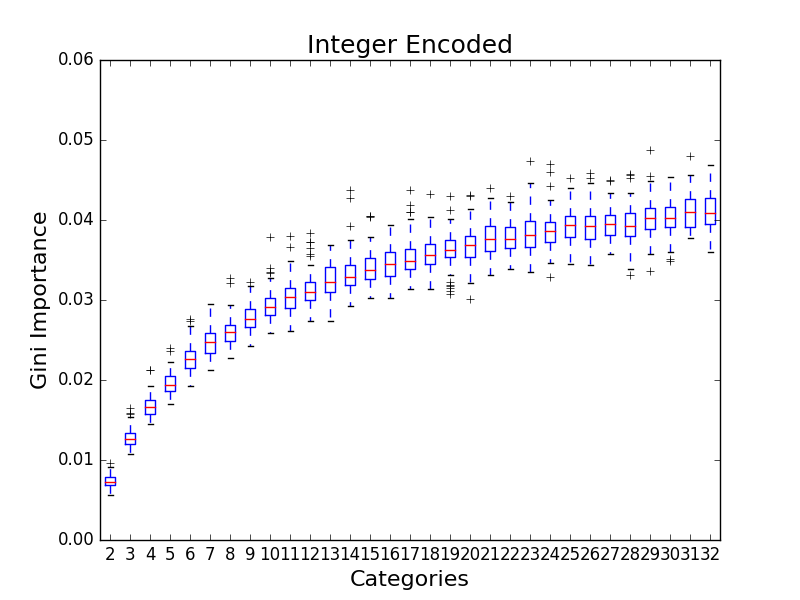
\includegraphics[width=\textwidth]{figures/random_forests/rf_bias_integer}
    \caption{Integer Encoded}
    \label{fig:integer}
  \end{subfigure}
  ~
  \begin{subfigure}[b]{0.45\textwidth}
    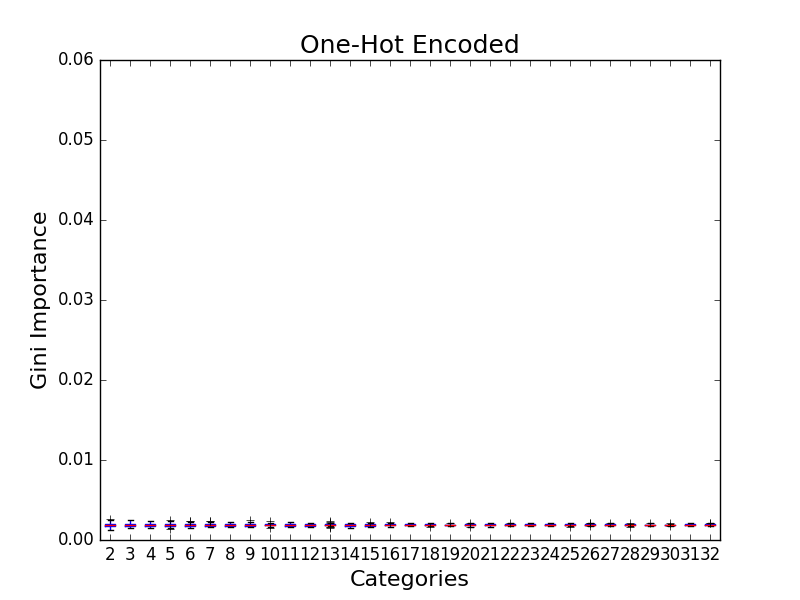
\includegraphics[width=\textwidth]{figures/random_forests/rf_bias_onehot}
    \caption{One-Hot Encoded}
    \label{fig:one-hot}
  \end{subfigure}
  \caption{Comparison of effect of encoding schemes for categorical variables on variable importance scores. The variables have randomly-chosen values with no correlation with output labels and 2-32 categories.}
  \label{fig:encoding-schemes}
\end{figure}

\begin{figure}[h!]
  \centering
  \begin{subfigure}[b]{0.45\textwidth}
    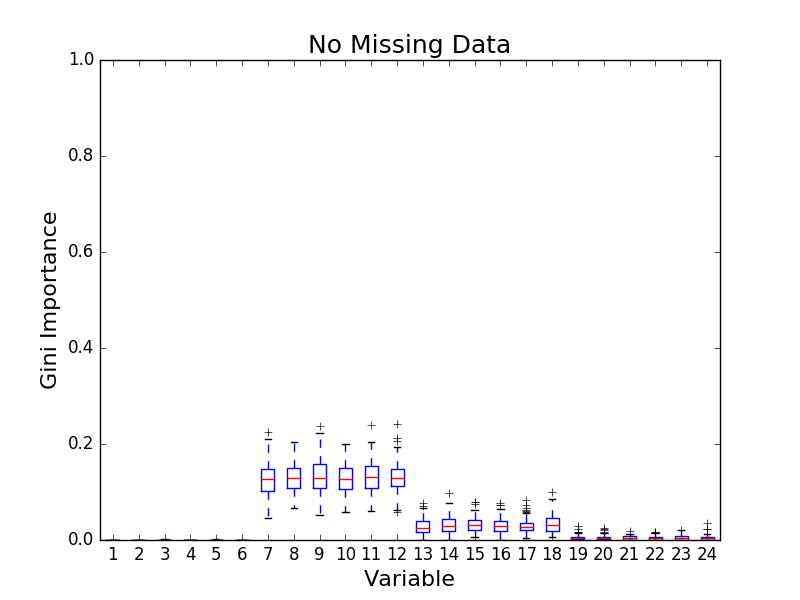
\includegraphics[width=\textwidth]{figures/random_forests/rf_missing_data_none}
    \caption{No Missing Data}
    \label{fig:missing-data-none}
  \end{subfigure}
  ~
  \begin{subfigure}[b]{0.45\textwidth}
    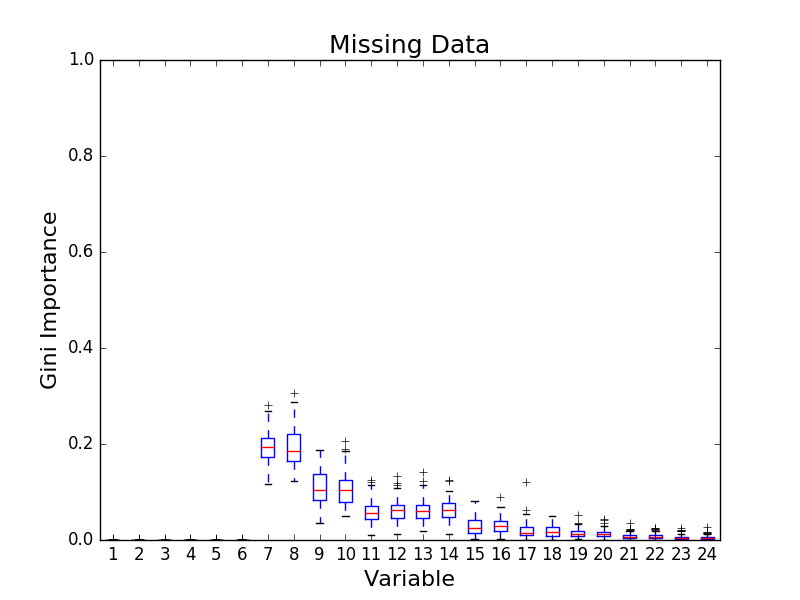
\includegraphics[width=\textwidth]{figures/random_forests/rf_missing_data}
    \caption{Missing Data}
    \label{fig:missing-data-missing}
  \end{subfigure}
  ~
  \begin{subfigure}[b]{0.45\textwidth}
    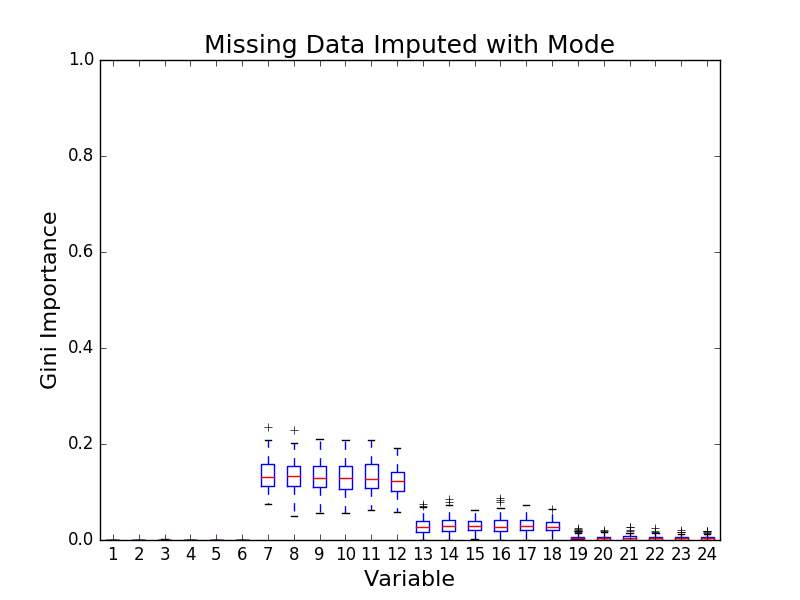
\includegraphics[width=\textwidth]{figures/random_forests/rf_missing_data_imputed_mode}
    \caption{Missing Data Imputed with Mode}
    \label{fig:missing-data-imputed}
  \end{subfigure}
  \caption{Effect of missing data on variable importance scores.}
  \label{fig:missing-data}
\end{figure}

\begin{figure}[h!]
  \centering
  \begin{subfigure}[b]{0.45\textwidth}
    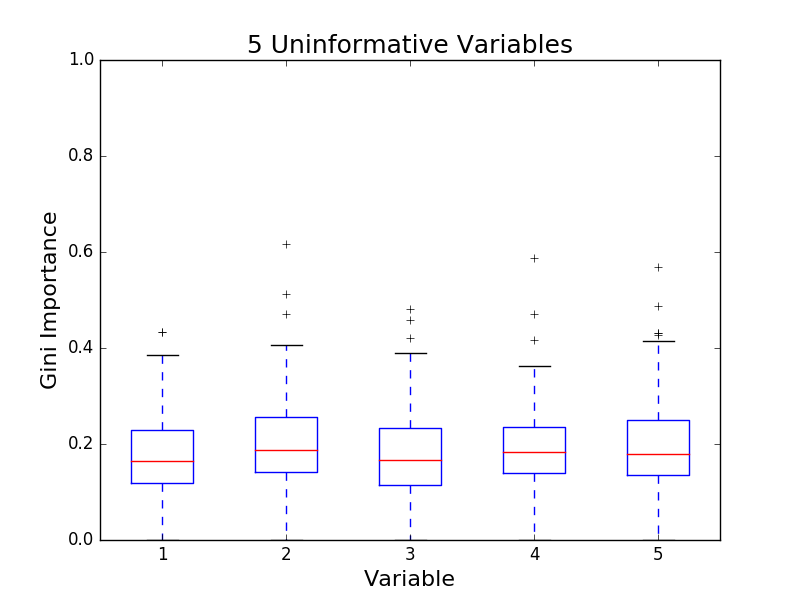
\includegraphics[width=\textwidth]{figures/random_forests/rf_variable_count_bias_5.png}
    \caption{5 Uninformative Variables}
    \label{fig:var-count-5}
  \end{subfigure}
  ~
  \begin{subfigure}[b]{0.45\textwidth}
    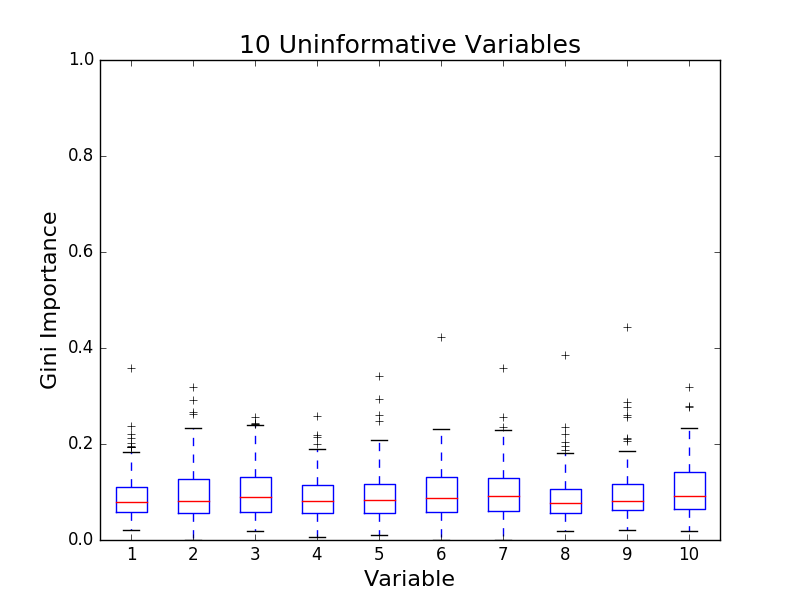
\includegraphics[width=\textwidth]{figures/random_forests/rf_variable_count_bias_10.png}
    \caption{10 Uninformative Variables}
    \label{fig:var-count-10}
  \end{subfigure}
  ~
  \begin{subfigure}[b]{0.45\textwidth}
    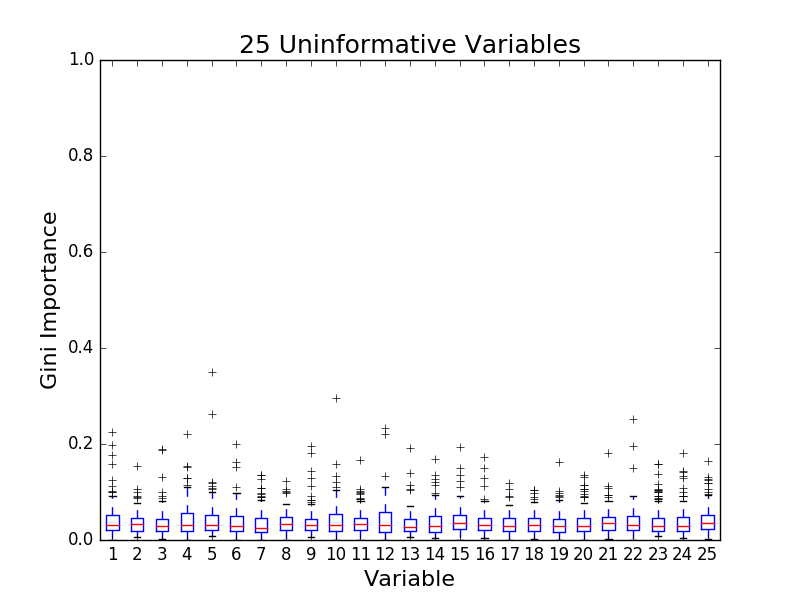
\includegraphics[width=\textwidth]{figures/random_forests/rf_variable_count_bias_25.png}
    \caption{25 Uninformative Variables}
    \label{fig:var-count-25}
  \end{subfigure}
  \caption{Distributions of variable importance scores with 5, 10, and 25 uninformative variables.}
  \label{fig:var-count}
\end{figure}

\begin{figure}[h!]
  \centering
  \begin{subfigure}[b]{0.45\textwidth}
    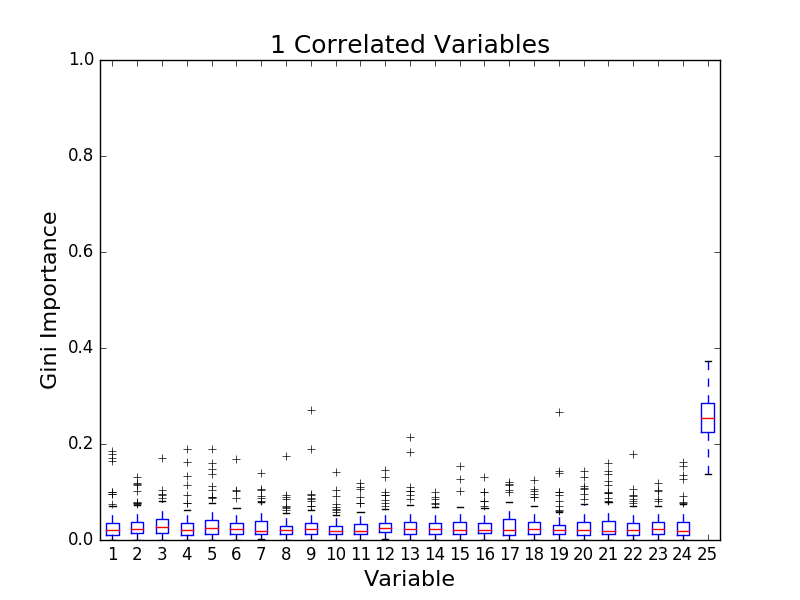
\includegraphics[width=\textwidth]{figures/random_forests/rf_correlated_1_0_1.png}
    \caption{1 Correlated Variable}
    \label{fig:corr-1-1}
  \end{subfigure}
  ~
  \begin{subfigure}[b]{0.45\textwidth}
    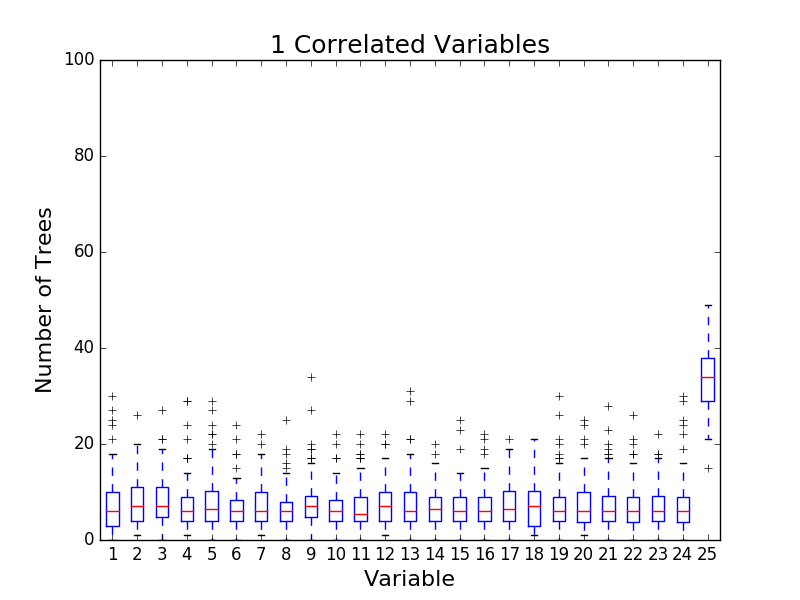
\includegraphics[width=\textwidth]{figures/random_forests/rf_correlated_1_0_1_feature_counts.png}
    \caption{1 Correlated Variable}
    \label{fig:corr-1-1-counts}
  \end{subfigure}
  ~
  \begin{subfigure}[b]{0.45\textwidth}
    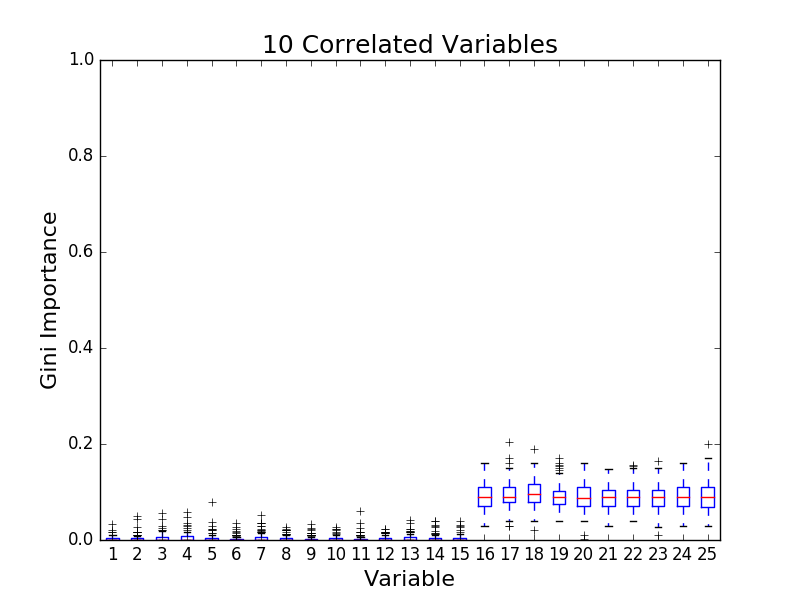
\includegraphics[width=\textwidth]{figures/random_forests/rf_correlated_1_0_10.png}
    \caption{10 Correlated Variables}
    \label{fig:corr-1-10}
  \end{subfigure}
  ~
  \begin{subfigure}[b]{0.45\textwidth}
    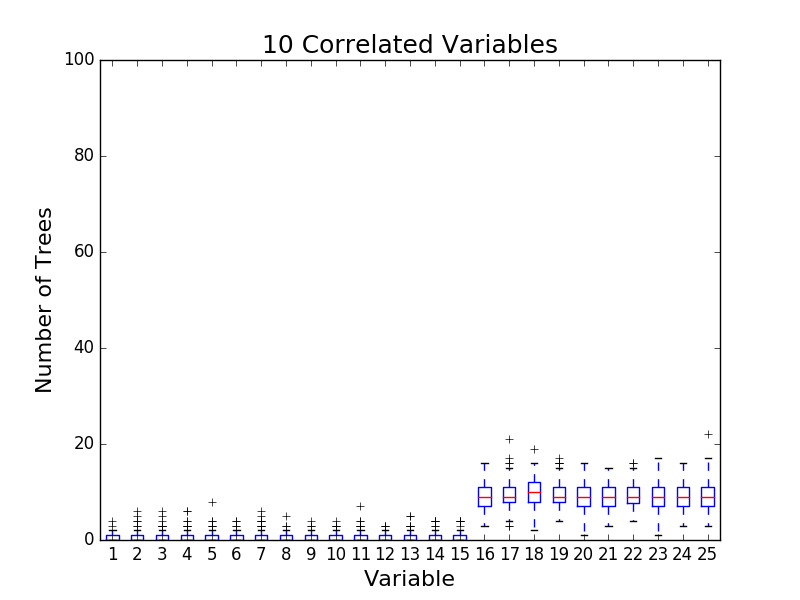
\includegraphics[width=\textwidth]{figures/random_forests/rf_correlated_1_0_10_feature_counts.png}
    \caption{10 Correlated Variables}
    \label{fig:corr-1-10-counts}
  \end{subfigure}
  ~
  \begin{subfigure}[b]{0.45\textwidth}
    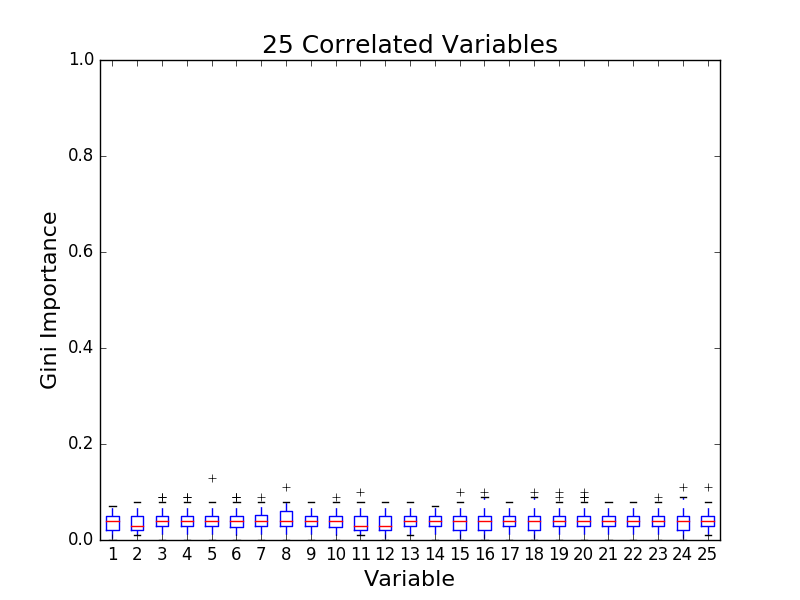
\includegraphics[width=\textwidth]{figures/random_forests/rf_correlated_1_0_25.png}
    \caption{25 Correlated Variables}
    \label{fig:corr-1-25}
  \end{subfigure}
  ~
  \begin{subfigure}[b]{0.45\textwidth}
    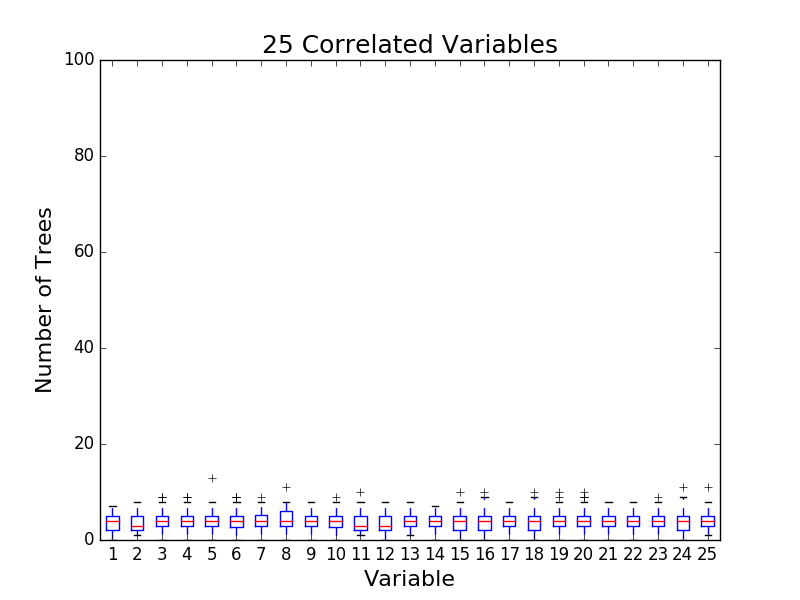
\includegraphics[width=\textwidth]{figures/random_forests/rf_correlated_1_0_25_feature_counts.png}
    \caption{25 Correlated Variables}
    \label{fig:corr-1-25-counts}
  \end{subfigure}
  ~
  \caption{Analysis of variables from generated data sets with 1, 10, and 25 out of 25 variables perfectly correlated with the output label. The left-hand side figures are distributions of variable importance scores. Right-hand side figures are number of trees using each variable.}
  \label{fig:corr-1}
\end{figure}



\begin{figure}[h!]
  \centering
  \begin{subfigure}[b]{0.45\textwidth}
    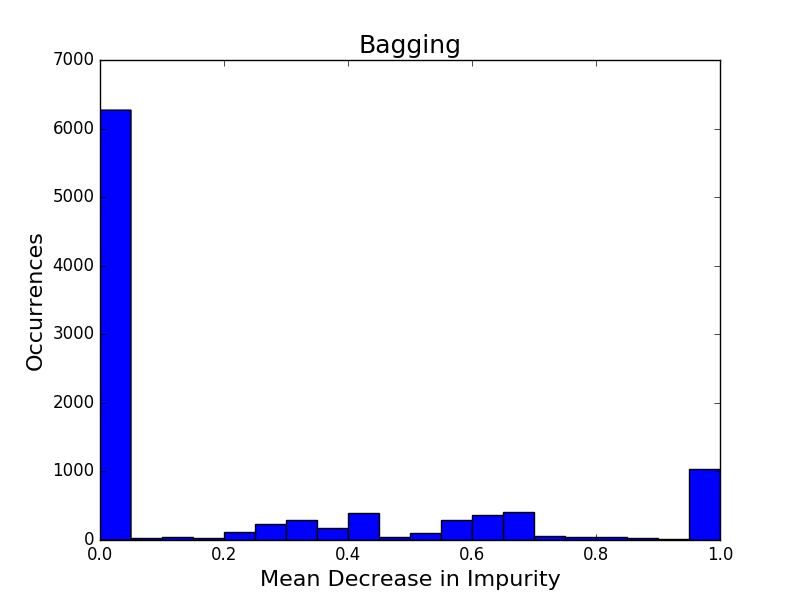
\includegraphics[width=\textwidth]{figures/random_forests/bagging_bias_bagging_hist.png}
    \caption{Bagging}
    \label{fig:bagging-bias-bagging}
  \end{subfigure}
  ~
  \begin{subfigure}[b]{0.45\textwidth}
    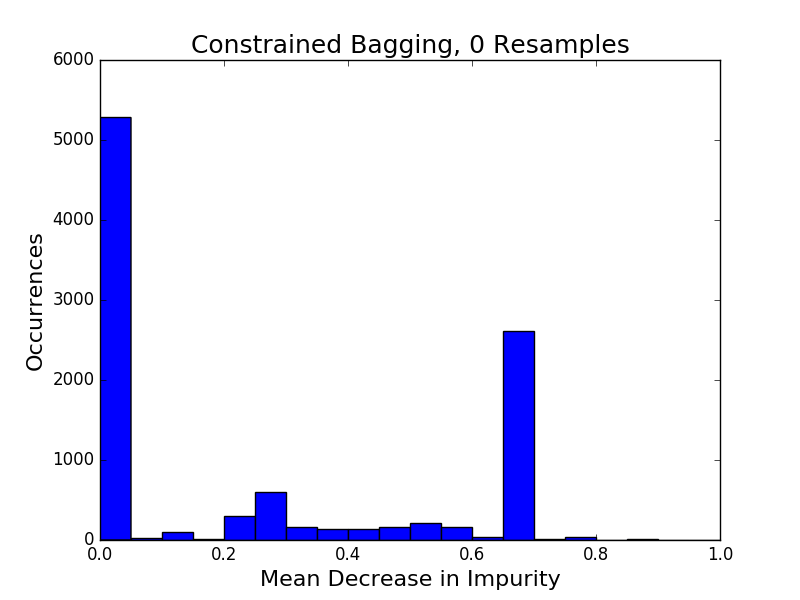
\includegraphics[width=\textwidth]{figures/random_forests/bagging_bias_no_bagging_hist.png}
    \caption{Constrained Bagging, 0 Resamples}
    \label{fig:bagging-bias-constrained-0}
  \end{subfigure}
  ~
  \begin{subfigure}[b]{0.45\textwidth}
    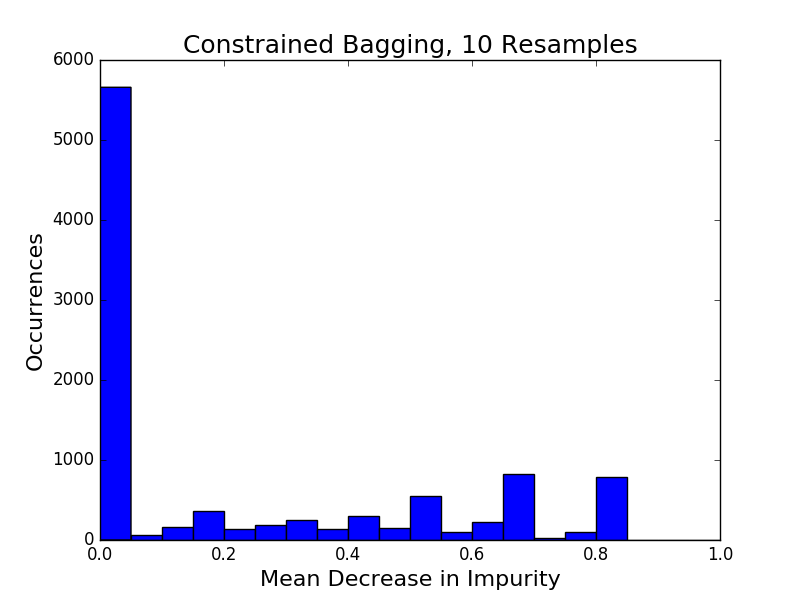
\includegraphics[width=\textwidth]{figures/random_forests/bagging_bias_constrained_bagging_hist_10.png}
    \caption{Constrained Bagging, 10 Resamples}
    \label{fig:bagging-bias-constrained-10}
  \end{subfigure}
  ~
  \begin{subfigure}[b]{0.45\textwidth}
    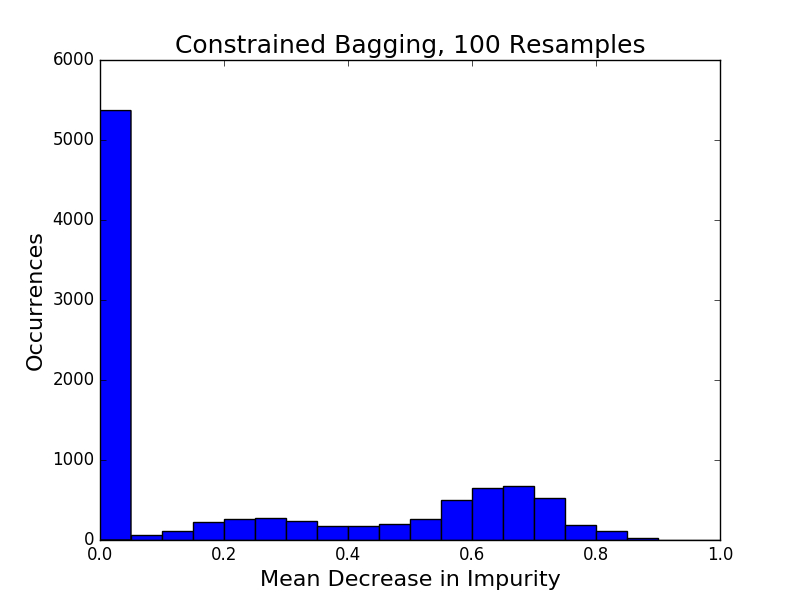
\includegraphics[width=\textwidth]{figures/random_forests/bagging_bias_constrained_bagging_hist_100.png}
    \caption{Constrained Bagging, 100 Resamples}
    \label{fig:bagging-bias-constrained-100}
  \end{subfigure}
  ~
  \begin{subfigure}[b]{0.45\textwidth}
    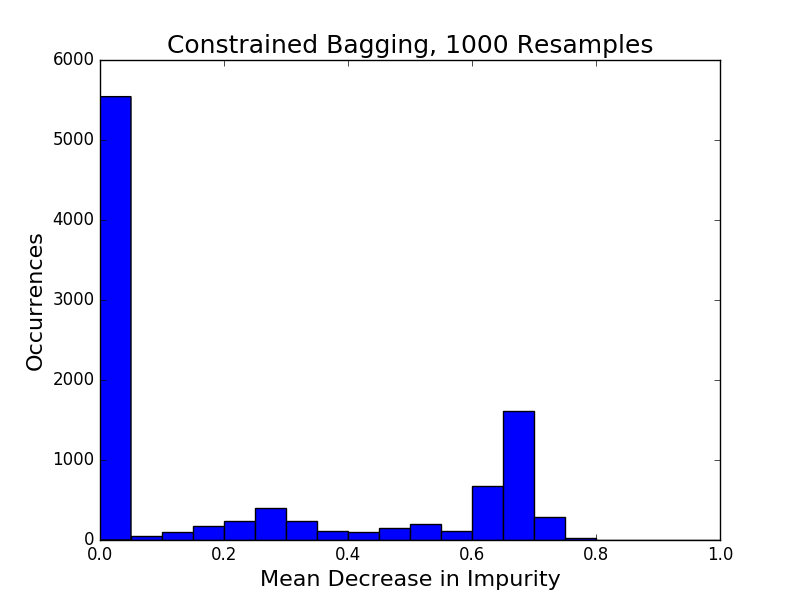
\includegraphics[width=\textwidth]{figures/random_forests/bagging_bias_constrained_bagging_hist_1000.png}
    \caption{Constrained Bagging, 1000 Resamples}
    \label{fig:bagging-bias-constrained-1000}
  \end{subfigure}
  ~
  \caption{Distributions of mean decreases in impurity when using bagging and constrained bagging with 0, 10, 100, and 1000 additional re-sampled instances.}
  \label{fig:bagging-bias}
\end{figure}

\section{Tables}
\begin{table}[h!]
  \begin{center}
    \begin{tabular}{ c c c}
      \hline
      \textbf{Group} & \textbf{Before} & \textbf{After}\\ \hline
      1 & A/T & A/T \\
      1 & A/T & A/T \\
      1 & A/T & A/T \\
      1 & X/X & A/T \\
      2 & T/T & T/T \\
      2 & A/A & A/A \\
      3 & A/A & A/A \\
      3 & X/X & X/X \\
    \end{tabular}
  \end{center}
  \caption{Examples of two groups with known and unknown genotypes, before and after imputation with a threshold frequency of 100\%.}
  \label{tab:unknown-genotypes-example}
\end{table}

\begin{table}[h!]
  \begin{center}
    \begin{tabular}{ c c c }
      \hline
      \textbf{Individual} & \textbf{(X, 1)} & \textbf{(X, 10)} \\ \hline
      1 & A/T & X/X \\
      2 & T/T & C/C \\
    \end{tabular}
  \end{center}
  \caption{Examples of SNP values for two individuals.  The SNPs are labeled by pairs of chromosome and position.}
  \label{tab:encoding-example-snps}
\end{table}

\begin{table}[h!]
  \begin{center}
    \begin{tabular}{ c c c c c c c }
      \hline
      \textbf{Individual} & \textbf{X, 1, A/A} & \textbf{X, 1, T/T} & \textbf{X, 1, A/T} & \textbf{X, 10, C/C} & \textbf{X, 10, G/G} &\textbf{X, 10, C/G} \\ \hline
      1 & 0 & 0 & 1 & 0 & 0 & 0 \\
      2 & 0 & 1 & 0 & 1 & 0 & 0 \\
    \end{tabular}
  \end{center}
  \caption{Feature matrix for the SNPs of the two individuals in Table~\ref{tab:encoding-example-snps}.  The features are labeled by triplets of chromosome, position, and genotype.}
  \label{tab:encoding-example-features}
\end{table}


\chapter{\uppercase{Conclusion}}


\appendix
\section{A Domain-Driven, Generative Data Model for BigPetStore}

\subsection{Abstract}
Generating large amounts of semantically-rich data for testing big data workflows is paramount for scalable performance benchmarking and quality assurance in modern machine-learning and analytics workloads.  The most obvious use case for such a generative algorithm is in conjunction with a big data application blueprint, which can be used by developers (to test their emerging big data solutions) as well as end users (as a starting point for validating infrastructure installations, building novel applications, and learning analytics methods).

We present a new domain-driven, generative data model for BigPetStore, a big data application blueprint for the Hadoop ecosystem included in the Apache BigTop distribution. We describe the model and demonstrate its ability to generate semantically-rich data at variable scale ranging from a single machine to a large cluster.  We validate the model by using the generated data to answer questions about customer locations and purchasing habits for a fictional targeted advertising campaign, a common business use case.

\subsection{Introduction}
Big data applications process large, dynamic, multidimensional data sets with the general goal of information and knowledge extraction.  With the wide variety of big data tools available and lagging documentation, both developers and users of big data systems benefit from the availability of realistic example applications.  For developers, such applications are useful for testing, benchmarking, and evaluating design choices; for users, example applications provide starting points for learning methods, developing their own applications, and implementing new analytics workflows.

BigPetStore is one such big data application blueprint built around processing transaction data for a fictional chain of pet stores.  BigPetStore targets the Hadoop \cite{Hadoop} ecosystem with examples implemented for loading, cleaning, aggregating, and performing analytics on data using Hive \cite{Thusoo2010}, Pig \cite{Olston2008,Gates2009}, and Mahout \cite{Mahout}. BigPetStore has been incorporated into the open-source Apache BigTop distribution \cite{BigTop}, where it is used for testing and as a reference application. One of BigPetStore's key features is the ability to scale from a single machine to a large cluster, making it easy to develop projects on a local machine and transfer the application to a large cluster for production testing.

To achieve the project's goals of providing high-quality, realistic examples, BigPetStore requires semantically-rich, complex data. At its core, BigPetStore relies on a generative data model for producing synthetic transaction data. Despite the growing number of real data sets now publically available, synthetic data generators have a number of advantages for BigPetStore over real data sets. The synthetic data generator can be packaged with BigPetStore, avoiding the cost, time, and infrastructure needed to host, transfer, and store large data sets. Synthetic data generators are scalable, allowing the user to choose how much data to generate -- a requirement for supporting BigPetStore's goal of running on both single machines and large clusters.  Licensing and privacy issues are avoided with the use of synthetic data sets. And lastly, the generated data can be customized by the user, allowing the user to generate data with specific criteria amenable to testing.  For example, a user may generate transactions from a small number of purchasable items so that clustering results can be easily visualized.

A variety of approaches for generating synthetic data sets exist.  TeraGen and the Intel Hadoop Benchmark Suite \cite{Huang2010} are popular tools that can generate data sets quickly and at any scale, but the resulting data is semantically-void and not useful for much more than simple benchmarks.  Multiple frameworks exist for generating synthetic data sets that satisfy relational database schemas \cite{Ghazal2013,Rabl2011a,Frank2012,Rabl2011,Gray1994,Bruno2005,Hoag2007}, and several approaches even provide domain-specific languages \cite{LogSynth,Bruno2005,Hoag2007} for specifying additional constraints (such as which distributions to sample from and allow for modeling basic relationships between fields using simple arithmetic equations \cite{Alexandrov2012}).

Recent work has addressed some aspects of the need for more dynamic data set generation: Arasu, et al. \cite{Arasu2011} demonstrated that constraint-solving techniques could be used as an alternative to procedural approaches. Such frameworks allow for reproducing the structural properties of real data, but the frameworks are not expressive enough to describe the dynamic generation processes and latent variables that would be needed to embed the desired informational complexity and rich semantics needed for BigPetStore's analytics examples.

Realizing the difficulty in creating a generic framework capable of modeling the semantics of real data, recent work\cite{Alexandrov2013} has focused on generating synthetic data sets that satisfy characteristics learned from real reference data. Such approaches appear promising but will need to overcome the difficulties of accurately training models, especially on raw data instead of features.

Until such purely generic methods reach maturity, BigPetStore's needs are best met by a customized, domain-driven model. Another example of such a model is The Information Discovery and Analysis System (IDAS) Data Set Generator (IDSG) \cite{Jeske2005,Lin2006}. IDSG was developed to test the effectiveness of IDASs in identifying potential terrorism threat scenarios using synthetic data.  Like BigPetStore, the developers of IDSG needed to avoid licensing restrictions and privacy issues associated with real data.

BigPetStore's current model has been used successfully to generate terabytes of synthetic data and is used regularly for testing in Apache BigTop, showcasing the value of the approach.  The current model is limited, however, in its ability to generate data that is semantically rich, limiting progress on BigPetStore's goals of providing realistic analytics examples.

In this work, we present a new domain-driven model and simulation method for BigPetStore.  Compared with BigPetStore's previous data generator, our model and implementation can generate data which contains geospatial, temporal, and quantitative features, similar to the type of data which businesses and organizations might typically encounter.  Combining the features of the TeraGen (scalability)  and MovieLens \cite{MovieLens} (semantically rich) input data sets commonly used for big data benchmarking, we present a synthetic data set generator which can be used to benchmark lower level tasks (such as sorting) as well as higher level tasks (such as clustering, recommending, and search indexing) at arbitrary scale.  To demonstrate that the model generates data with desirable properties, we performed an example analysis designed to guide a fictional advertising campaign (a typical business use case). The model's implementation was made available as open source software.

\subsection{Overview of Model \& Simulation Procedures}
Our generative model combines various well-known mathematical modeling techniques to simulate the factors affecting customers' purchasing habits.  Each part of the model is derived from \emph{ab initio} assumptions.  In several cases, real data is used to parameterize parts of the model. 

\subsubsection{Description of Generated Data}
The model generates data for four types of records: stores, customers, transactions, and transaction items (Figure~\ref{fig:relational-data-model}).  Store records contain both a unique identifier and a location in the form of a 5-digit zip code. Customer records consist of a unique identifier, a name, and a location given as a 5-digit zip code. Transaction records consist of a transaction identifier, a customer identifier, a store identifier, and a time given in days since the beginning of the simulation. Transaction item records contain a transaction identifier and an item description.  The item description is a list of key-value pairs stored as a string.  Key-value pairs are used since item characteristics differ depending on the type of item.  For example, dog food has a brand, a flavor, a size (in lbs), and a per-unit cost, while poop bags have a brand, a color, a count, and a per-unit cost.

\begin{figure}[!t]
  \centering
  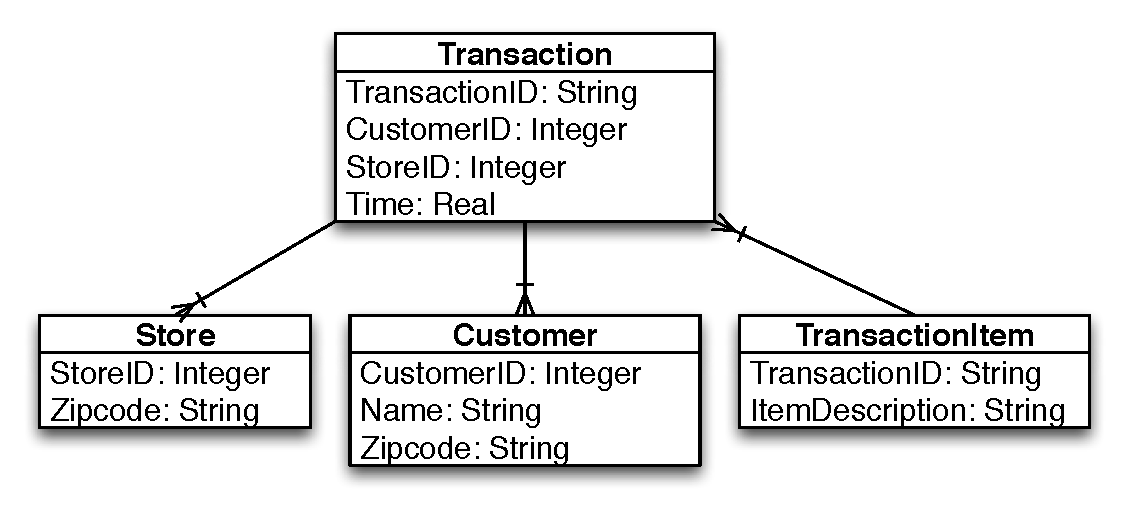
\includegraphics[width=3.5in]{figures/bigpetstore/transactions_data_model.eps}
  \caption{Relational Data Model for Generated Data}
  \label{fig:relational-data-model}
\end{figure}

\subsubsection{Generation of Stores}
The locations of the stores are modeled by a probability density function (PDF) that gives the probability that a store's location is the given zip code. We designed the PDF to give to zip codes in high-population, high-income areas the highest probabilities. The PDF is composed of two individual PDFs. One PDF determines the probability of each zip code as the population of that zip code over the total population:

\begin{equation*}
p(\text{location}=z | \text{population}(z)) = \frac{\text{population}(z)}{\sum_{i} \text{population}(i)}
\end{equation*}

The second PDF scales the probabilities of the zip codes by their incomes.  The zip code with the highest-income has a probability $s$-times larger than that of the lowest-income zip code. The values in-between are interpolated using an exponential function:

\begin{equation*}
p(\text{location}=z | \text{income}(z)) = s ^ {\big( \frac{\text{income} - \min_i{\textrm{income}(i)}} {\max_i{\textrm{income}(i)} - \min_i{\textrm{income}(i)}} - 1 \big)}
\end{equation*}

The combined PDF is given as: 

\begin{align*}
p(\text{location}=z) = &Z p(\text{location}=z | \text{population}(z)) \\
&p(\text{location}=z | \text{income}(z))
\end{align*}

where $Z$ is the normalization factor.  Given the small size ($\approx$30,000 zip codes) of the data set, $Z$ can be found directly by iterating over all of the zip codes and summing the scores. The population and household income data for the zip codes were taken from from the U.S. Census American Community Survey \cite{ACS}.  The stores' locations are generated by sampling zip codes from the PDF.

\subsubsection{Generation of Customers}
For each proposed customer location zip code $z$, we compute the distance $d_m(z)$ between $z$ and each store's zip code $s_z$ to find the closest store.  The zip codes' latitudes and longitudes (taken from the Zip Code Database Project \cite{Zips}) are used to compute the distances. Each zip code $z$ is assigned a weight $w_z$ according to its distance $d_m(z)$ to the nearest store using an exponential distribution with the average distance $\beta$:

\begin{align*}
&w_z = \beta^{-1} \exp(-\beta^{-1} \, d_m(z)) \\
&d_m(z) = \min_{s_z} \, d(z, s_z)
\end{align*}

The customer's zip code is chosen by sampling from the zip codes with the probabiltiy of choosing each zip code $z$ proportional to its weight $w_z$.

Names are generated using data from the Name Database\cite{NameDB}. Each record in the database gives a name, a weight, and flag indicatings if the name can be used as a first name, a last name, or both.  PDFs generated for the first and last names using the weights.  The customer's name is generated by sampling a first name and a last name from each PDF respectively.

We determine the number of pets $N_p$ each customer has by sampling from a discrete uniform distribution of integers. We then sample the number of dogs $N_d$ as a discrete uniform distribution of integers between 0 and $N_p$.  The remaining number of pets are assigned to be cats.

\begin{align*}
N_c = N_p - N_d \\
N_d \sim U(0, N_p) \\
N_p \sim U(1, b)
\end{align*}

\subsubsection{Simulation of Transactions}
A transaction simulation is run for each customer. The transaction's store is set to the store located closest to the customer.  Transaction times are generated from a Monte Carlo process that proposes transaction times based on the usage of the customer's items and Poisson processes modeling the amount of time between the customer visiting the store and running out of the items (Section~\ref{sec:transaction-times}).  The purchased items are generated by a Hidden Markov Model (HMM) parameterized by the transaction time and amount of time remaining for the items in the customer's inventory (Section~\ref{sec:transaction-purchases}).

\begin{figure}[!t]
  \centering
  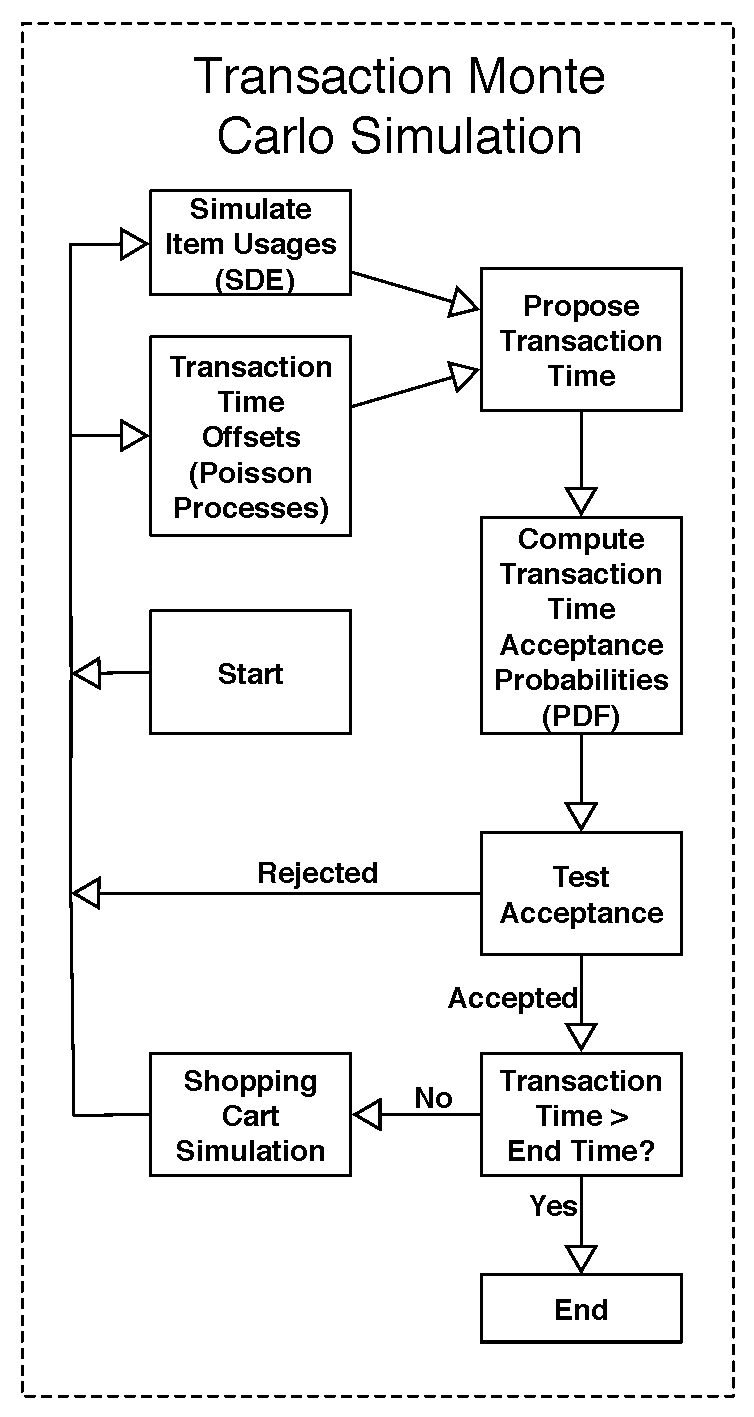
\includegraphics[width=3.5in]{figures/bigpetstore/transaction_simulation.eps}
  \caption{Flowchart of Transaction Monte Carlo Simulation}
  \label{fig:trans_sim}
\end{figure}

\subsubsection{Simulation of Transaction Times} \label{sec:transaction-times}
Transaction times are simulated using a Monte Carlo method (Figure~\ref{fig:trans_sim}).  The usage over time of each item category is simulated. Items categories are groups of items which are interchangeable such as ``dry dog food,'' ``dry cat food,'' and ``kitty litter.'' The time between the customer's visit to the store to buy more items in each category and the exhaustion time of that item category is modeled using a Poisson process. Proposed transaction times for each item category are computed based on the exhaustion time and time sampled from the Poisson process. The earliest transaction time is taken as the overall proposed transaction time.  The probability of the transaction time is calculated using a PDF.  If rejected, new transaction times are proposed.  Otherwise, the purchased items are modeled using a separate process (discussed below). After the items are chosen, the process begins again with the simulation of the item category usages.

In the first stage of the process, the usage of items over time is modeled using a stochastic differential equation (SDE):

\begin{equation*}
\frac{da_i}{dt} = \min \{-\mu_i + \sigma_i\, dW_i(t), 0\}
\end{equation*}

where $a_i$ is the amount of item category $i$ ``stuff'' remaining at time $t$. The variable $\mu_i$ gives the average usage rate and $\sigma^2_i$ gives the variance of the usage rate for item category $i$. The SDE is numerically integrated using the Euler-Maruyama method\cite{Klouden13} with time step $\Delta t_n$ sampled from an exponential distribution:

\begin{align*}
&a_{n+1, i} = a_{n,i} - \min \{\mu_{i, c} \, \Delta t_n + \sigma_{i, c} \, \sqrt{\Delta t_n} R_n, 0.0\} \\
&t_{n+1} = t_n + \Delta t_n \\
&\Delta t_n \sim \text{Exp}(\beta^{-1}_{i,c}) \\
&R_n \sim \text{N}(0, 1)
\end{align*}

where $a_{n, i}$ is the amount remaining of item category $i$ at time step $t_n$, $\mu_{i,c}$ is the average amount used per time used, $\sigma^2_{i,c}$ is the variance of the amount used per time used, and $\beta_{i,c}$ is the item category's average amount of time between uses for customer $c$.  The parameters $\mu_{i, c}$, and $\sigma^2_{i,c}$ are computed from a base rate for each item category multiplied by the number of pets of the appropriate species the customer $c$ has.  The exhaustion time $T_{E,i}$ for each item category is found by simulating the usage until $a_{n,i} \leq 0$.

The proposed transaction time is found from the exhaustion times (Eq.~\ref{eq:transaction-times}).  For each item category, the offset time $T_{O, i}$ between when a customer would visit the store and the exhaustion time is sampled from an exponential distribution. The distribution is parameterized by $\beta_c$, the average number of days before triggering a transaction. The parameter $\beta_c$ is set separately for each customer $c$ by sampling from a uniform distribution. A proposed transaction time $T_{P, i}$ for each item category is found by subtracting the offset time $T_{O, i}$ from the exhaustion time $T_{E, i}$.  The earliest proposed transaction time is taken as the overall proposed transaction time $T_T$.

\begin{align} \label{eq:transaction-times}
&T_T = \min_i \, \{  T_{P, i}\} \\
&T_{P, i} = T_{E,i} - T_{O, i} \nonumber\\
&T_{O, i} \sim \text{Exp}(\beta^{-1}_c) \nonumber \\
&\beta_c \sim \text{U}(a, b) \nonumber
\end{align}

The acceptance probability $p(t_{n+1}=T_T|t_n)$ of the proposed transaction time $T_T$ is modeled using a PDF (Eq.~\ref{eq:transaction_time_pdf}). For now, the PDF only ensures that the proposed transaction time is more recent than the last transaction time.

%The PDF could be extended to incorporate additional factors including time-dependent events such as sales, weather, and the amount of money the customer has available at the time.

\begin{equation} \label{eq:transaction_time_pdf}
p(t_{n+1}=T_T|t_n) = \left\{ 
  \begin{array}{l l}
   1 & \quad t_{n+1} \geq t_n\\
   0 & \quad t_{n+1} < t_n
  \end{array} \right.
\end{equation}

The proposed transaction time is accepted if $p(t_{n+1}=T_T) < r$, where $r \sim \text{U}(0, 1)$. Until the proposed transaction time is accepted, a new proposed transaction time is generated by sampling new offset times. If the proposed transaction time is accepted, the purchased items are chosen through a separate simulation discussed in Section~\ref{sec:transaction-purchases} below. Transactions are generated until the accepted transaction time is later than the end time given as a simulation parameter.

\begin{figure*}[!t]
  \centering
  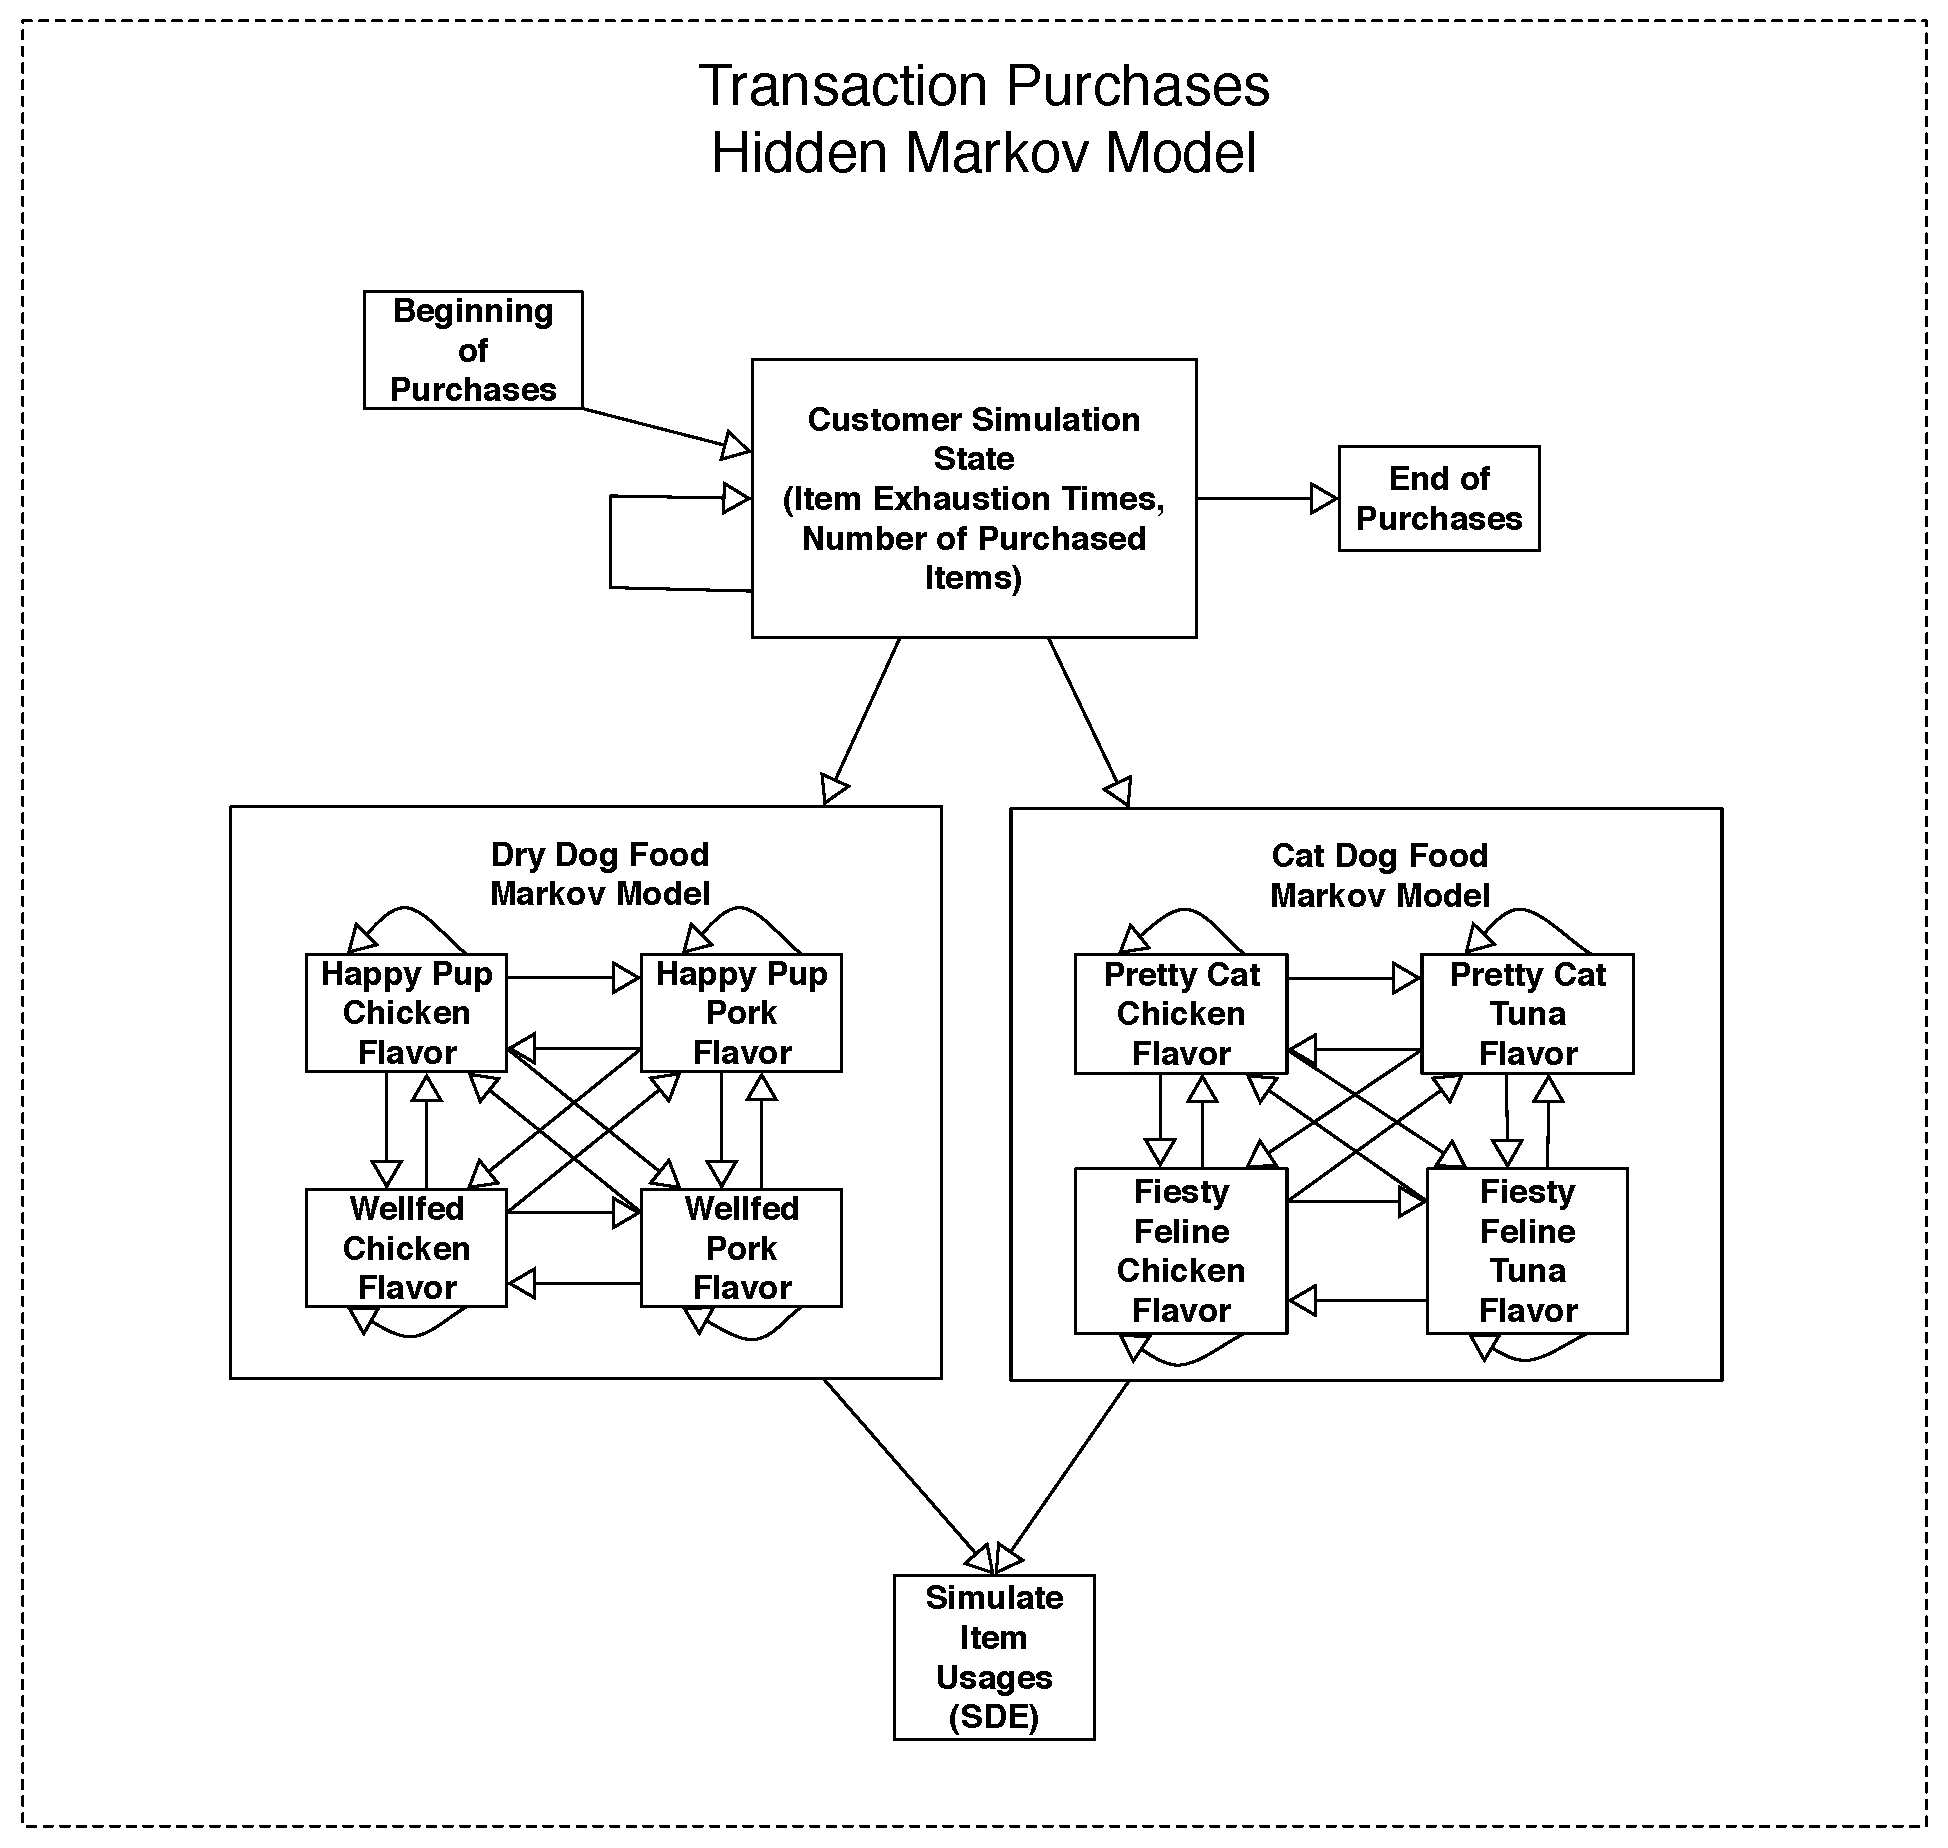
\includegraphics[width=6in]{figures/bigpetstore/shopping_cart_simulation.eps}
  \caption{Example Shopping Cart Hidden Markov Model}
  \label{fig:shopping_cart_sim}
\end{figure*}

\subsubsection{Simulation of Transaction Items} \label{sec:transaction-purchases}

A customer's purchases in each transaction are modeled using a layered Hidden Markov Model (HMM) (Figure~\ref{fig:shopping_cart_sim}).  The HMM has three types of states: the start state, the purchase states, and the stop state. There are an infinite number of purchase states, parameterized by the exhaustion times of the customer's item categories and the transaction time.

The observables of the states correspond to the item categories.  Each item category $i$ is assigned a weight $w_i$ according to the amount of time between the transaction time $T_t$ and $T_{E,i}$ when each item category will be exhausted (based on the usage simulations):

\begin{align} \label{eq:category-weights}
&w_i = - \beta^{-1}_c \exp(-\beta^{-1}_c (T_{E, i}- T_T)) \\
&\beta^{-1}_c \sim U(a,b) \nonumber
\end{align}

where $\beta_c$ the average number of days between when a customer purchases an item and the exhaustion time. The value $\beta_c$ is set separately for each customer by sampling from a uniform distribution. The value $w_i$ is used to model the propensity for a customer to purchase an item they will run out at time $T_{E, i}$ in the future when at the store at time $T_T$.

The item category is chosen by sampling from the item categories with the probability of choosing each item category $i$ proportional to its weight $w_i$.

Markov Models are used to model the customer's purchasing behavior for each item category.  Each state $X_n$ corresponds to an item in that category. The customer's buying habits are determined by the transition probabilities:  

\begin{align}
Pr(X_{n+1}&=x|X_n=y) = \nonumber \\
& \left\{ 
  \begin{array}{l l}
   (1.0 - p_l) \, Pr(x,y)  & \quad \text{if $x \neq y$}\\
   p_l & \quad \text{if $x = y$}
  \end{array} \right.
\end{align}

where $w_l$ is the loopback probability, giving the probability of choosing the same item $y$ again. The function $Pr(x,y)$ gives the probability of choosing the item $x$ given that the previous item was $y$:

\begin{equation*}
Pr(x,y) = \frac{\sum_f w_f w_{f,s}(x, y)}{\sum_{j \neq x} \sum_f w_f w_{f,s}(x, j)}
\end{equation*}

where $w_f$ is the weight of a particular field $f$.   The pair of items $x$ and $y$ are weighted  according to the equality of the values for each field:

\begin{equation*}
w_{f,s}(x,y) = \left\{ 
  \begin{array}{l l}
   w_{f,s}  & \quad \text{if $x$.$f$ = $y$.$f$}\\
   1 - w_{f, s} & \quad \text{if $x$.$f$ $\neq$ $y$.$f$}
  \end{array} \right.
\end{equation*} 

The weights $w_l$, $w_f$, and $w_{f, s}$ are chosen randomly for each customer:

\begin{align*}
&w_l \sim N(\mu, \sigma^2) \\
&w_f \sim N(\mu, \sigma^2) \\
&w_{f, s} \sim N(\mu, \sigma^2)
\end{align*}

If the weights are greater than 1, they are rounded down to 1.  Likewise, if the weights are less than 0, they are rounded up to 0.

To simulate an item purchase, the chosen Markov model is transitioned forward by one state. The current states of the Markov models are kept between purchases.  After an item is chosen, the item category's exhaustion time is updated by propagating the item category usage SDE described in Section~\ref{sec:transaction-times}, resulting in an implicit creation of the next possible purchase state in the HMM.

After each purchase, the HMM's current state is transitioned to either the new purchase state or the stop state.  The probability of choosing the next state is 

\begin{align*}
&Pr(X_{n+1}=\text{stop}|X_n) = p(\text{stop})\\
&Pr(X_{n+1}=\text{purchase}|X_n) = 1 - p(\text{stop})
\end{align*}

where $p(\text{stop})$ is the probability of choosing the stop state and is given by

\begin{equation*}
 p(\text{stop}) = \frac{w_{\text{stop}}}{w_{\text{stop}} + \sum_i w_i}
\end{equation*}

where $w_{\text{stop}}$ is the weight of the stop state and is a simulation parameter and the weight $w_i$ of each item category $i$ was given earlier in Eq.~\ref{eq:category-weights}.

If the stop state is chosen, the transaction is finished and the next transaction is started according to the procedure presented in Section~\ref{sec:transaction-times}.

%The HMM can be extended to consider additional factors such as the amount of money spent so far in the transaction and the customer's spending habits.

\subsection{Implementation}
The models and simulations were implemented using Python. The source code is available at \url{https://github.com/rnowling/bigpetstore-data-generator} under the Apache Public License v2.

\subsection{Evaluation of the Model}
In accordance with our original design goals, we evaluated the model and implementation in terms of their abilities to generate semantically-interesting data and scale from a single local machine to a cluster.

\subsubsection{Example Analysis of Generated Data}
To evaluate the semantic content of the generated data, we performed two example analyses in support of a fictional advertising campaign using data for 10 stores, 10,000 customers, and five years of transactions generated from the model. The analyses were designed to be realistic and driven by real-world business concerns.  Due to limited advertising budgets, businesses need to decide who to target and what sort of advertisements are likely to be effective for each type of customer.  We analyzed data generated from the model to determine where the advertising campaigns should be targeted geographically and identify customer purchasing profiles.

First, we wanted to identify how close most customers live to a store since advertising to people who live or work too far away from a store is unlikely to be effective and will increase our costs. We analyzed the distribution of distances between customers' homes and their nearest stores.  We found that most customers tend to live within 15 miles of their closest store, suggesting that we should limit our advertising to a 15-mile radius around each our store.

\begin{figure}[!t]
  \centering
  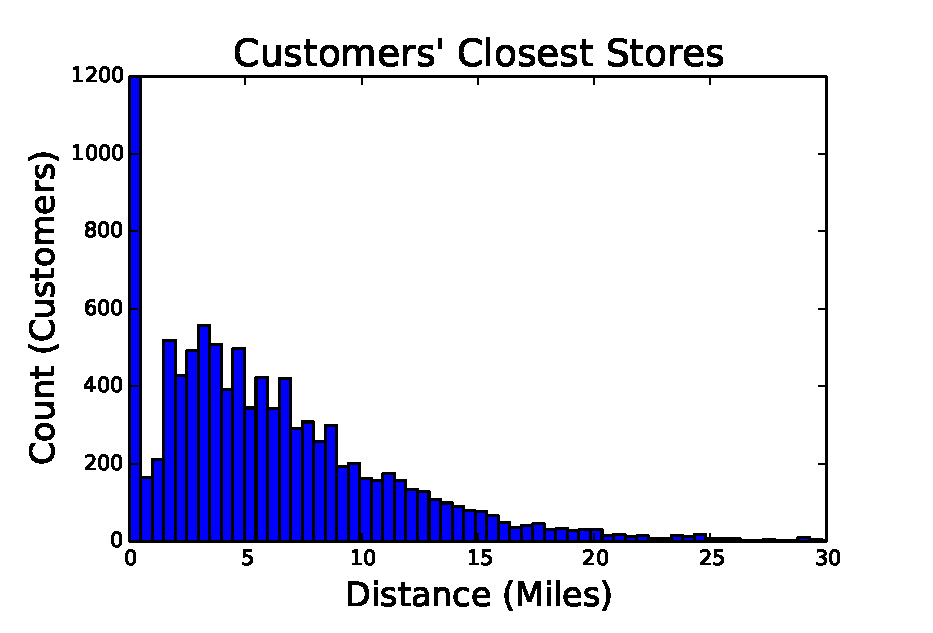
\includegraphics[width=3.5in]{figures/bigpetstore/customer_store_distances.eps}
  \caption{Distributions of Distances of Customers to Closest Stores}
  \label{fig:cluster_analysis}
\end{figure}

Secondly, we profiled our customers' purchasing habits to optimize the advertising campaign's effectiveness by customizing the advertised products for each customer.  For each customer, we generated a feature vector by computing the frequency with which they would purchase the same brand or flavor from one transaction to the next.  We clustered the customers' feature vectors using the KMeans algorithm with a range of cluster counts. Twenty clusters converged the error.

\begin{figure}[!t]
  \centering
  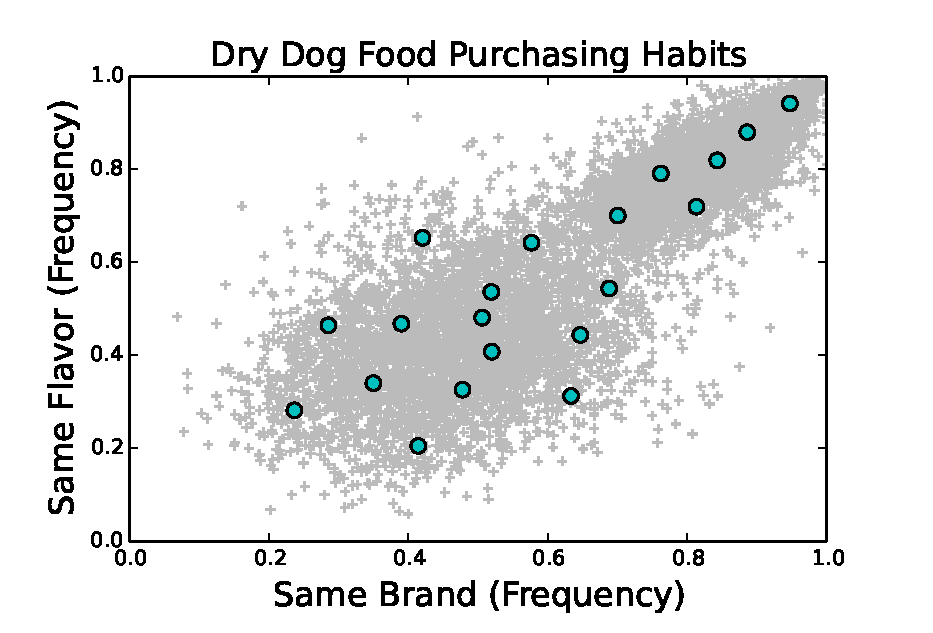
\includegraphics[width=3.5in]{figures/bigpetstore/cluster_analysis.eps}
  \caption{Clustering of Brand and Flavor Purchasing Preferences. Grey plus signs (+) represent customer data points, and cyan circles represent cluster centers.}
  \label{fig:cluster_analysis}
\end{figure}

Analysis of the feature vectors and clusters revealed four predominant purchasing profiles (Figure~\ref{fig:cluster_analysis}).  High frequencies of purchasing the same flavors repeatedly were tightly-correlated with high frequencies of purchasing the same brands -- these customers were likely to be happy with a particular item and kept purchasing the same item repeatedly.  For our advertising campaign, it would be unlikely to get these customers to purchase different items, so we should create incentives to purchase larger quantities, especially when inventory levels are high and needed to be depleted.  Other customers had a tendency to purchase either the same flavor or brand repeatedly, but varied in their choice of the other.  For customers who prefer a particular brand, we should target our advertising campaign to suggest other flavors sold by that brand.  Likewise, for customers who prefer a particular flavor, we should target our advertising campaign to suggest other brands with that flavor.  Lastly, some customers had very low frequencies of purchasing neither the same brand nor flavor.  Other factors, such as cost, not represented in this analysis may be driving these customers' purchasing habits and will need further study.


\subsubsection{Scaling of Data Size and Run Time}
BigPetStore aims to scale from a local desktop to a large cluster. To evaluate the scaling of the model and implementation, we benchmarked the data generator on a laptop with a 2 GHz Intel Core i7 CPU, 8 GB of RAM, and a 256 GB SSD using the Python implementation with a single thread. Using the test setup, between 1,500 and 2,000 transactions can be generated per second (Table~\ref{tab:benchmarks}). As the customers' transaction simulations are independent of one another, the transaction generation can easily be parallelized so that 1,500-2,000 transactions can be generated per thread per second.

\begin{table}[!t]
%% increase table row spacing, adjust to taste
\renewcommand{\arraystretch}{1.3}
% if using array.sty, it might be a good idea to tweak the value of
% \extrarowheight as needed to properly center the text within the cells
\caption{Benchmarks of Data Generator}
\label{tab:benchmarks}
\centering
%% Some packages, such as MDW tools, offer better commands for making tables
%% than the plain LaTeX2e tabular which is used here.
\begin{tabular}{|p{0.75cm}||p{1.2cm}||p{1cm}||p{1.25cm}||p{1cm}||p{1cm}|}
\hline
Stores & Customers & Simulated Time (years) & Transactions & Data Size (MB) & Run Time (min)\\ \hline
10 & 10,000 & 1 & 279,870 & 18 & 3.5 \\ \hline
%10 & 100,000 & 1 & 
100 & 10,000 & 1 & 279,586 & 18 & 3.5 \\ \hline
% 100 & 100,000 & 1 & 
10 & 1,000 & 5 & 123,309 & 8 & 1.1 \\ \hline
100 & 1,000 & 5 & 127,064 & 8 & 1.2 \\ \hline
10 & 10,000 & 5 & 1,275,542 & 84 & 11.0 \\ \hline
%10 & 100,000 & 5 & 
100 & 10,000 & 5 & 1,268,403 & 84 & 10.5 \\ \hline
\end{tabular}
\end{table}

The number of transactions (and hence, data size) grows as $O(N_c T)$ where $N_c$ is the number of customers and $T$ is the amount of time to be simulated. The amount of data generated can be scaled as large as necessary simply by increasing $N_c$ and $T$. Five years of transactions for 100,000 customers will generate approximately 1 GB of data. A terabyte of data can be generated by simulating 100 million customers over five years. 

\subsection{Discussion and Conclusion}
We have described a domain-driven mathematical model and accompanying simulation for generating semantically-rich data.  We validated the method by analyzing generated data to inform decisions in a fictional advertising campaign. Scalability testing combined with analysis of the implementation suggests that the data generation method can scale from small data sets appropriate for desktop development to large data sets for testing and benchmarking of clusters. We have released the implementation source code under the open-source Apache Public License v2.

We see many opportunities for building on the work presented.  We intend to expand the model to incorporate additional factors.  Deeper integration of existing fields such as location and purchasing profiles (e.g., to model regional purchasing preferences) will increase the variety of the semantic information encoded in the generated data. The incorporation of weather and climate data can be used to influence when customers shop, the types of products they buy, and the amount of products purchased. For example, customers would be less likely to shop during snow storms, more likely to buy items such as winter apparel for their pets, and more likely to purchase bulk quantities to reduce the number of transactions. Modeling of time-dependent events such as sales, evolution of customer purchasing profiles over time, and ``life events,'' such as the birth or passing of pets, will enable more interesting time-series analysis of the data.  We would also like to expand the scope of the model to incorporate business processes (such as inventory management, customer complaints, employees, etc.), thus enabling queries about the relationship between internal business process and customer behavior.

The current implementation was prototyped in Python.  We are finishing a Java implementation that can be used from the command-line, Hadoop, and Spark, enabling massive parallelization and improved scaling.  As part of the effort to re-write the framework in Java, we are abstracting classes for statistical modeling and simulation for reuse in developing data generators for other domains. We will commit the resulting implementation to BigPetStore hosted in the Apache BigTop distribution to enable ease of access and immediate benefit to current users. 

\subsection{Acknowledgments}
The authors would like to thank Brian P. Clare and Casey Robinson for useful and interesting discussion.  Will Benton, Trevor M. Cickovski, Erik Erlandson, Scott A. Hale, Hank Jakiela, Casey Robinson, and Douglas Thain provided invaluable feedback on the manuscript.  JV would like to thank the Apache BigTop community for their interest in and support of BigPetStore.  The authors would also like to thank Matt Fenwick, Nigel Savage, and Bhashit Parikh for their contributions to BigPetStore. The authors would like to thank Red Hat, Inc. and the University of Notre Dame for their support of this work.

\backmatter

\bibliography{thesis}
\bibliographystyle{abbrvnat}

\end{document}

